%# -*- coding: utf-8-unix -*-
%%==================================================
%% chapter01.tex for SJTU Master Thesis
%%==================================================

%\bibliographystyle{sjtu2}%[此处用于每章都生产参考文献]
\chapter{系统实验与验证}\label{chap:sys_eval}
在本章中,我们对本文提出的主动式容器云资源管理模型进行实验验证,并对实验结果进行必要的分析和说明。本文提出的模型可以分为负载监测和预测、资源供给和管理以及负载应对这三个部分。由于本文的最终目标是提高容器云应对负载变化的响应能力,优化的方法主要分为基于预测的主动式调整和对任务实例分发调度策略的优化,资源供给部分主要职责是根据预测和观测的资源使用量确认实例规模大小,并没有任何优化的功能,因此我们验证的重点也主要是在负载预测的准确性和引入的新任务实例调度策略对容器云中任务实例分发管理的影响。在负责预测部分的实验中,我们根据实验得出相关模型的预测正确率和预测偏差率等数据,利用这两个量化标准来说明相应模型实际的预测效果;在负载优化部分的实验中,为了对本文提出的模型进行验证,我们利用Docker \emph{swarm}作为容器云的比较对象,并通过服务创建和服务伸缩的方法对本文实现的系统进行了相关实验。

\section{实验环境设定}\label{sec:env_prep}
为了验证系统的有效性,本课题对整体的硬件和软件环境进行了相关准备,具体设定如下所示:
\begin{enumerate}
\item 我们使用4台Dell R420机架式服务器作为容器云的托管服务器,利用Docker swarmkit作为底层容器集群实现,构建基于Docker的容器云。每台服务器有4个CPU核心,内存大小为8GB,详细的服务器硬件配置参数如表\ref{tb:machine_perf}所示。
\begin{table}[h]
\centering
\bicaption[tb:machine_perf]{物理服务器性能参数}{物理服务器性能参数}{Table}{Physical Server's Technical Specification}
\begin{tabular}{@{}lr@{}} \toprule
 资源类型 & 性能参数 \\ \midrule
 CPU型号 & Intel Xeon E5-2650\\
 CPU核心数 & 4\\
 内存大小 & 8G\\
 内网出入带宽 & 2Gbps\\
 外网出入带宽 & 100Mbps\\ \bottomrule
\end{tabular}
\end{table}
\item 整个容器集群利用上述4台服务器构成4个集群节点,包括1个管理者节点(manager)和3个工作者节点(worker)。在试验中,我们假定每台服务器的可用性指标保持一致,均为0.9,因此容器集群中每个节点的可用性也都保持一致。这意味着对同一个服务而言,任务在容器集群内任一节点上对服务的整体可用性的影响是一样的。
\item 在负载预测部分的实验中,我们使用1998年世界杯网站的流量数据作为模拟的系统负载数据,通过对该流量数据的预测结果来验证预测模块的有效性。该数据集包含了从1998年4月30日到1998年7月26日之间世界杯网站的访问请求记录,并且被广泛应用在了时序数据处理相关领域中,流量整体趋势如图\ref{fig:load_trend}所示:
\begin{figure}[htbp]
\centering
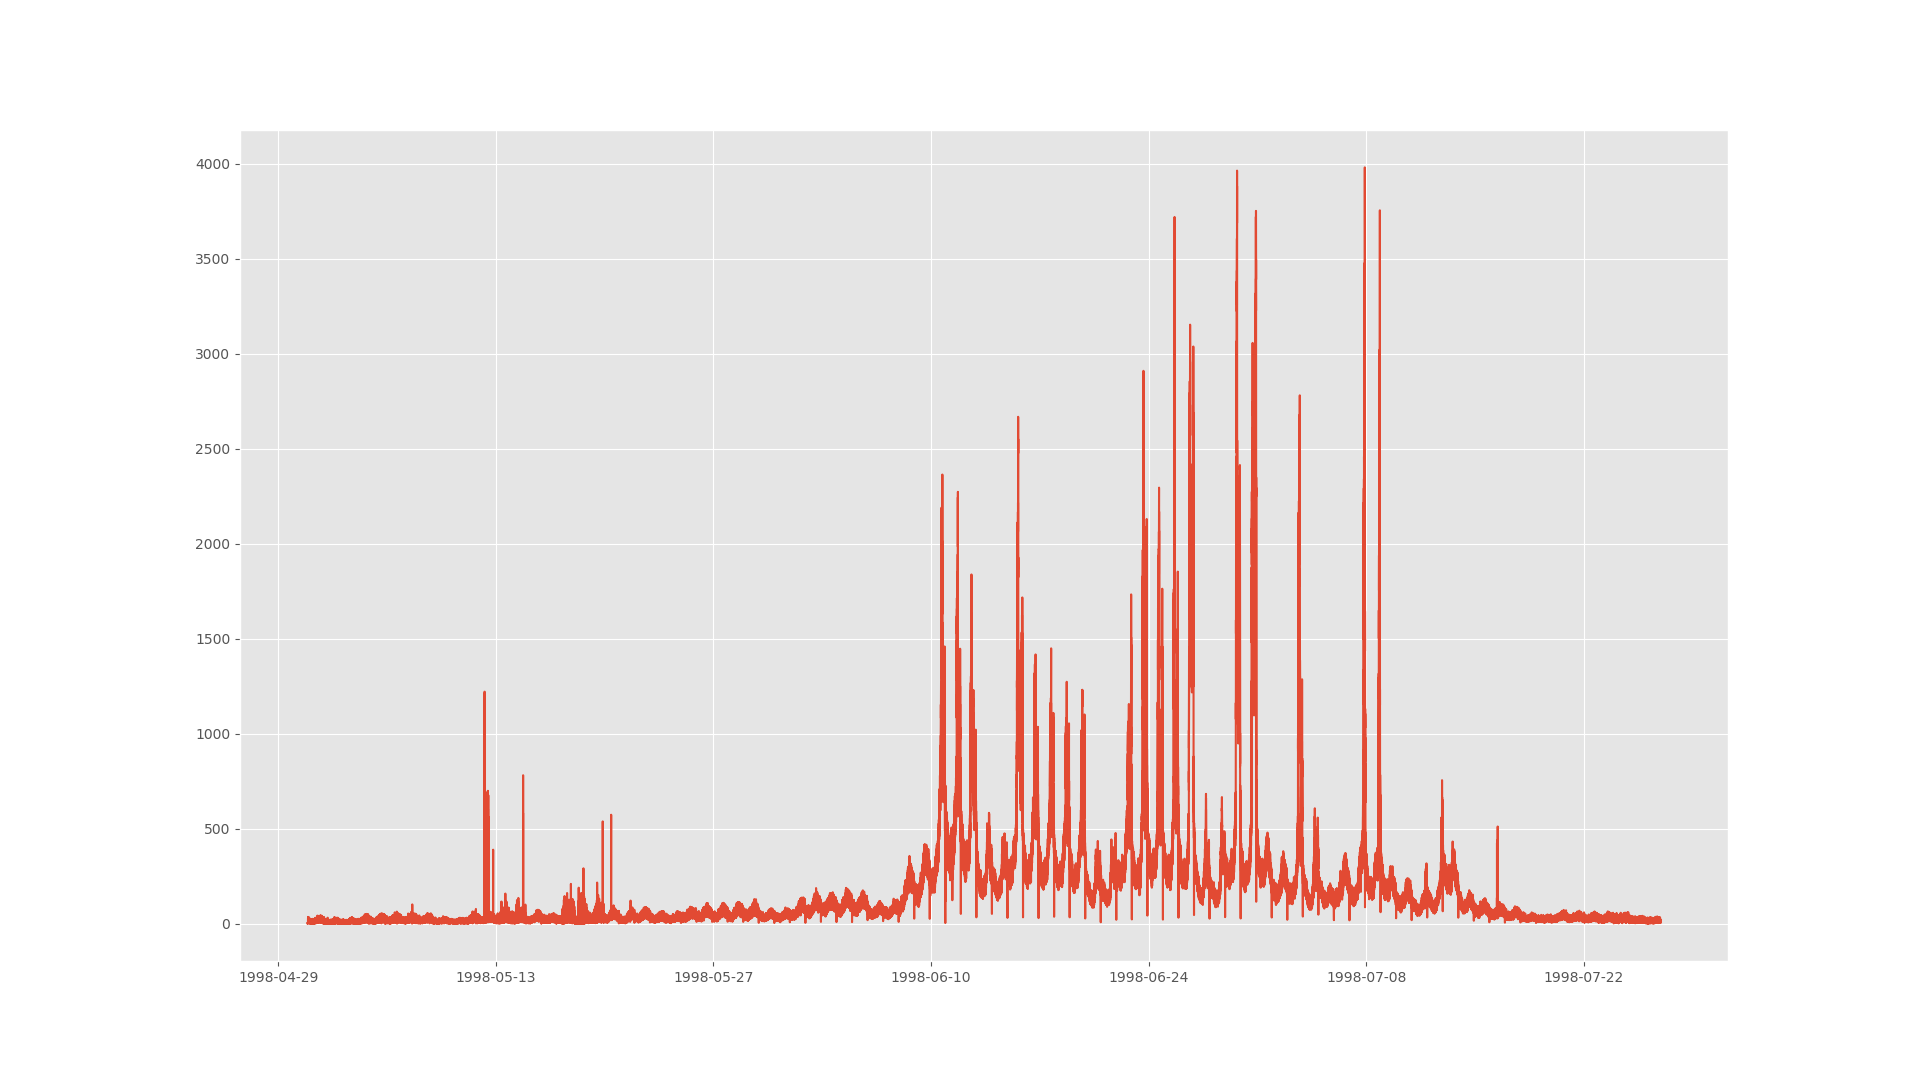
\includegraphics[width=0.9\textwidth]{./figure/alldata}
\bicaption[fig:load_trend]{98年世界杯网站整体流量趋势}{\textbf{98年世界杯网站整体流量趋势}}{Fig}{The load trend of 98' World Cup Site}
\end{figure}
\item\label{req:serv_image} 我们分别以Docker Hub上提供的官方\emph{debian:jessie}镜像和官方\emph{ubuntu:xenial}镜像为基础,通过依赖包安装的方式安装好\emph{Golang}的运行时环境(约270MB大小),构建两个不同的基础镜像\emph{base1}和\emph{base2}。我们分别基于这两个基础镜像对同一个\emph{Golang}应用构建两个不同的应用镜像\emph{image1}和\emph{image2}。除此之外,我们利用官方\emph{debian:jessie}镜像作为基础镜像,对shell应用构建了第三个应用镜像\emph{image3}。\emph{image1}和\emph{image3}都包含基础镜像\emph{debian:jessie},因此镜像\emph{image1}和镜像\emph{image3}中来自\emph{debian:jessie}镜像的层级文件可以被这两个镜像共享,这就意味着在同一个节点,只需要下载和安装一次\emph{debian:jessie}镜像,那相应的层级文件就能被镜像\emph{image1}和镜像\emph{image3}共享而不需要额外的下载。
\item 为了减少网络延迟和网络稳定性对试验的影响,我们选择使用Docker镜像的本地二进制文件安装方式来安装和配置依赖环境,而不是用诸如apt、yum等常见的依赖配置管理工具从网络上的官方二进制仓库来获取和安装相关依赖。
\item\label{req:serv_aval} 针对上述三个不同的应用镜像,我们在容器云中分别部署了三个不同的服务,分别命名为\emph{service1},\emph{service2}和\emph{service3},每个服务默认占用0.5个CPU核心和1GB的内存资源。每个服务指定的服务可用性目标是0.99。根据等式, 每个服务应该配置2个副本以满足服务可用性目标。
\item\label{req:registry_mirror} 为了减少网络传输的延迟,加快容器云整体的容器镜像分发速度,我们在实验环境下搭建了一个Docker \emph{registry}镜像来对镜像文件进行缓存和下载加速。Docker容器集群和Docker \emph{registry}服务之间通过百兆网络进行连接。容器集群中的各节点在下载镜像时可以利用本地搭建的Docker \emph{registry}服务进行下载,而避免直接从Docker Hub获得镜像导致的额外网络传输开销。
\item 为了获取更可信的数据,我们对每个实验项目进行三次独立实验,对测得实验数据去平均值作为该实验项目的观测值。在每次实验结束后,我们都将重启集群节点上的Docker Engine并重置整个实验环境,以避免下一次的实验收到本次实验过程的影响。
\end{enumerate}

\section{资源使用状态预测模块有效性验证}
由图\ref{fig:load_trend}中可以看出,流量的变化主要和比赛日时间有关,诸如工作日等日常的时间标志对流量变化的影响很小。比赛日之间的流量变化模式比较近似,而且在若干时间段内存在流量急速增加和迅速降低的场景。除此之外,通过对原始数据的分析,我们还发现每天不同时间段流量的变化基本是相似的。98年世界杯网站的数据集包括了从1998年4月30日到1998年7月26日之间网站的历史访问记录,而1998年世界杯的比赛日程为1998年6月10日到1998年7月12日。我们从整个样本集中选取了6月16日到7月9日之间世界杯网站的部分流量数据记录作为本次实验的预测评估数据集,分别利用基于整合移动平均自回归模型的预测算法和基于长短期记忆模型的预测算法在相应数据上进行预测,并给出相应的预测结果评估。

\subsection{基于整合移动平均自回归模型的预测实验}\label{sec:arima_eval}
在整合移动平均自回归模型模型的预测算法中,我们维护了一个4天的时间窗口。由于整合移动平均自回归模型的预测计算量随着时间窗口的增加而增加,我们将5分钟之内的资源使用状态进行汇总并计算出下一个周期的资源使用量预测。我们根据基于整合移动平均自回归模型的预测算法,对6月18日到6月19日之间、6月24日当天、7月8日到7月9日之间和7月11日到7月13日期间的流量数据进行预测,最终预测效果如图\ref{fig:arma_algo}所示:
\begin{figure}[htbp]
\centering
\subfigure[6月18日到6月19日]{
    \label{fig:arma_algo:5255}
    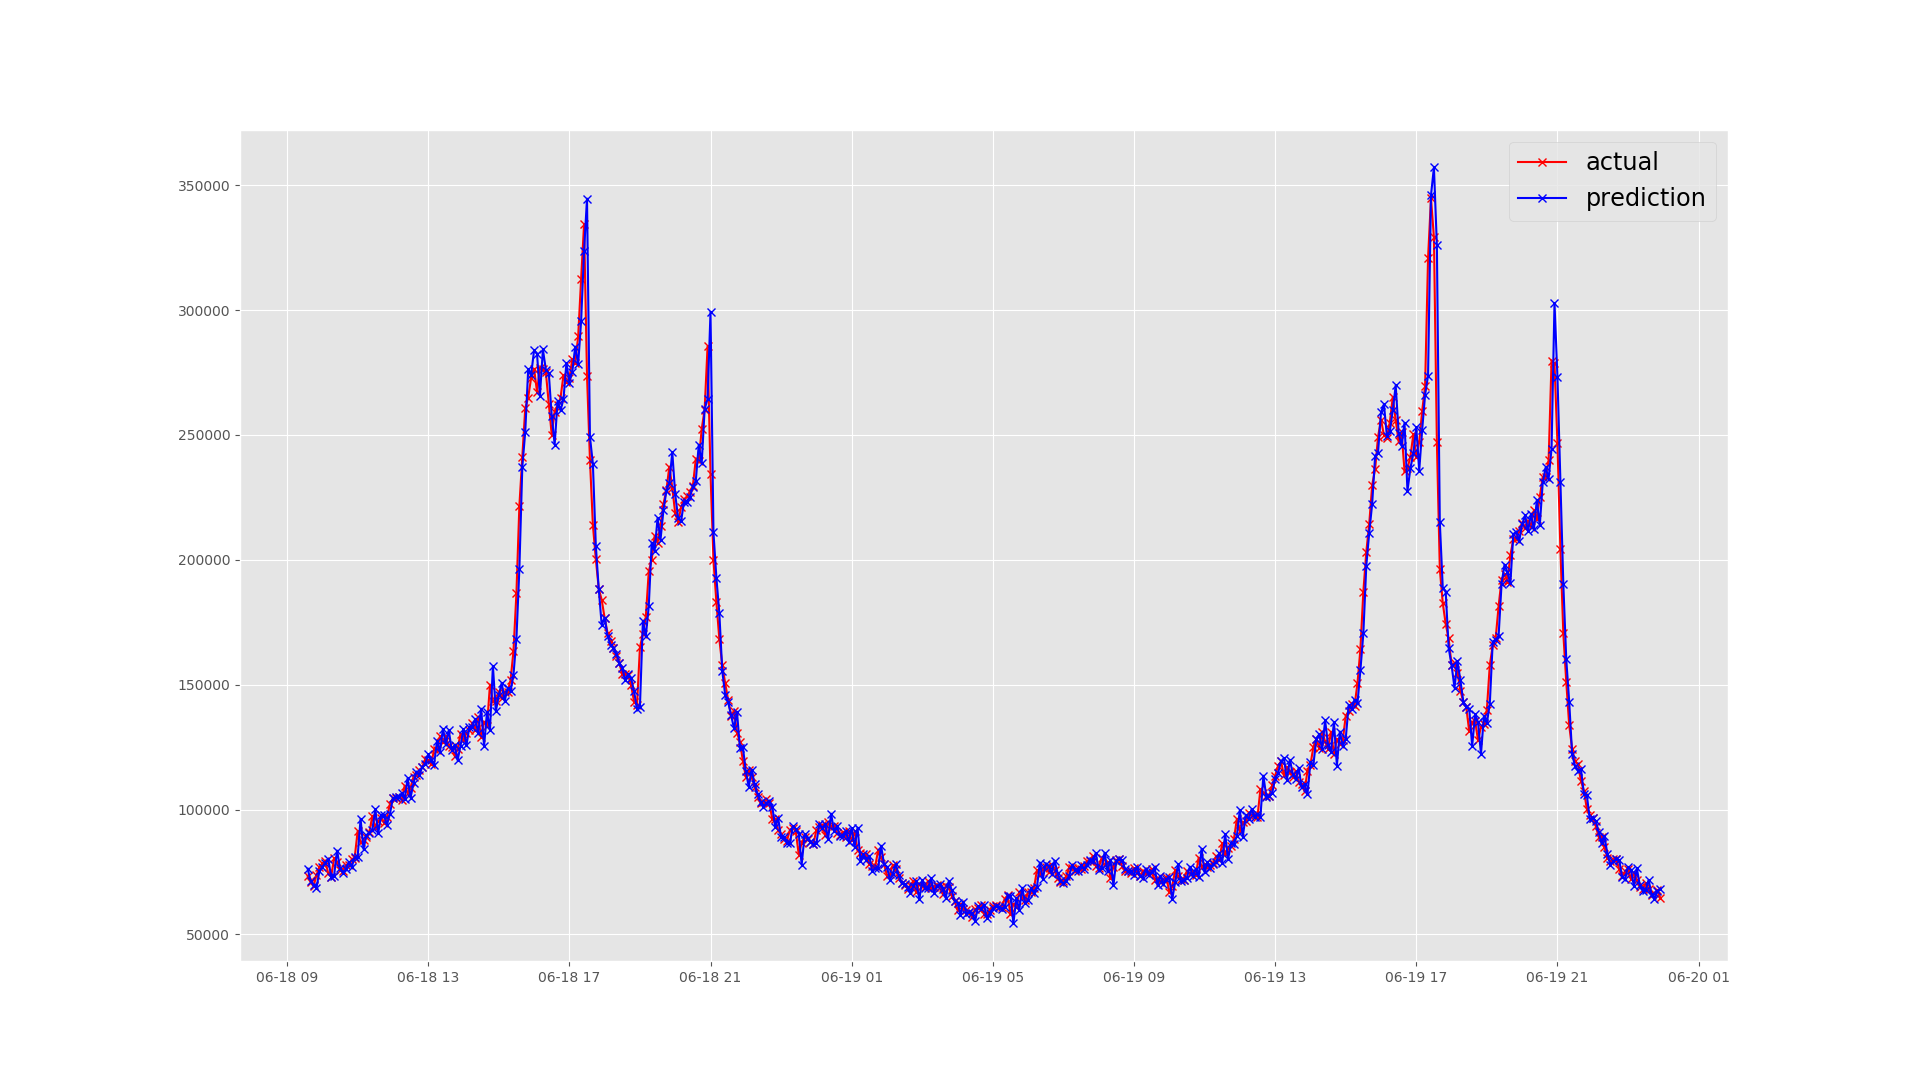
\includegraphics[width=0.45\textwidth]{./figure/arma5255}}
\subfigure[6月24日]{
    \label{fig:arma_algo:5961}
    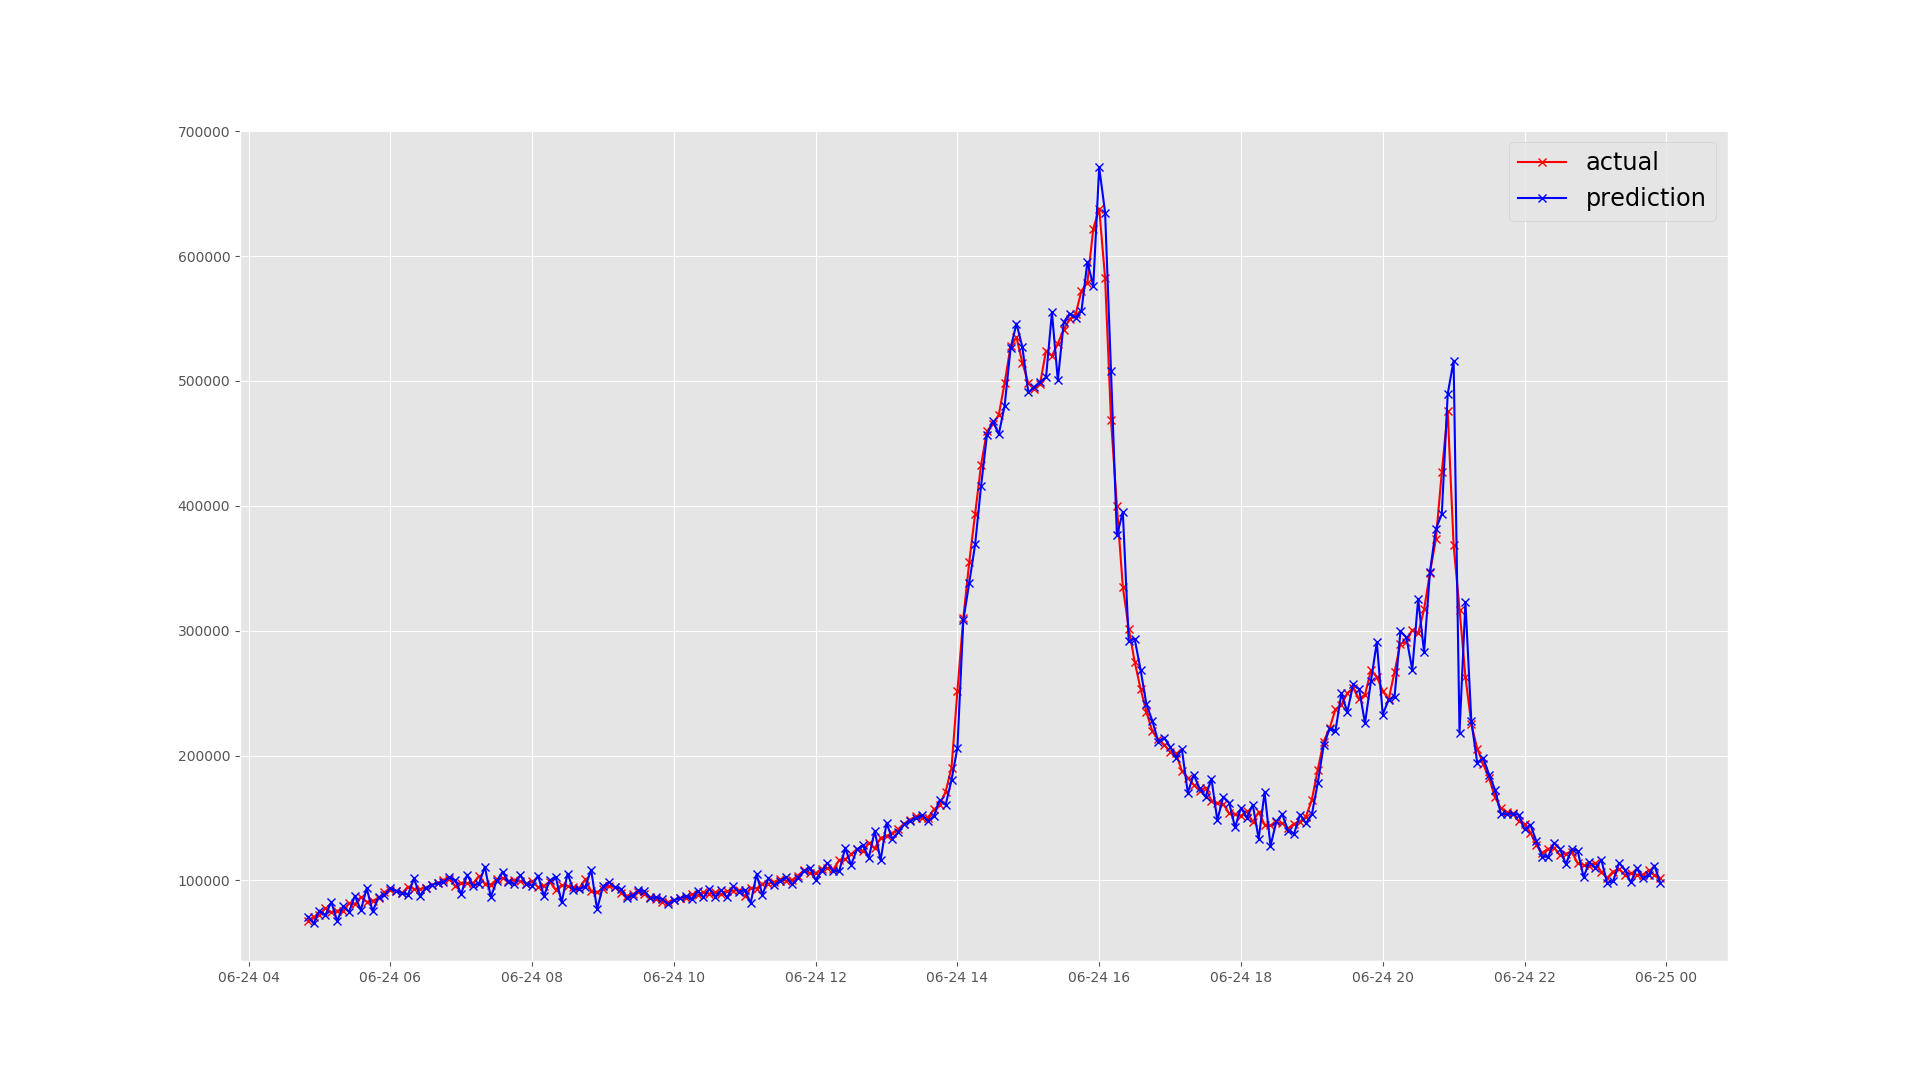
\includegraphics[width=0.45\textwidth]{./figure/arma5961}}
\subfigure[7月8日到7月9日]{
    \label{fig:arma_algo:7376}
    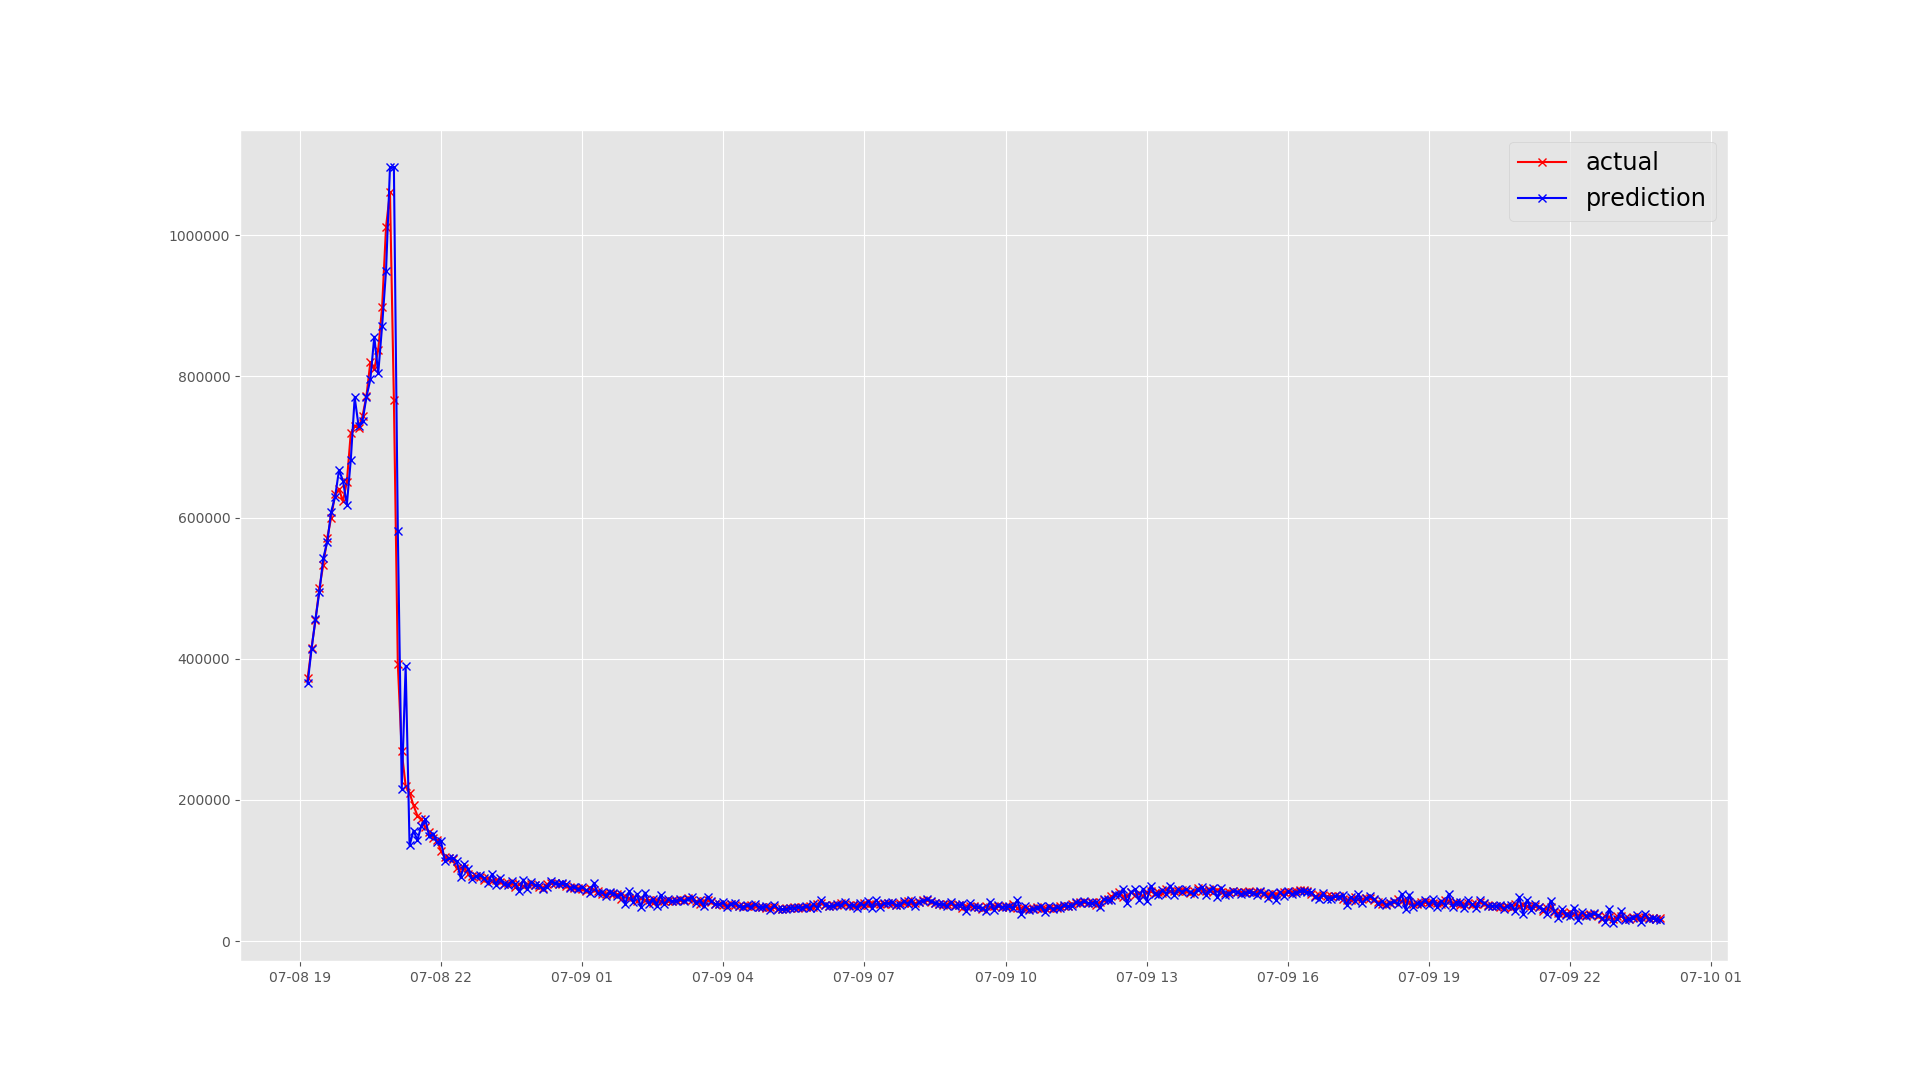
\includegraphics[width=0.45\textwidth]{./figure/arma7376}}
\subfigure[7月11日到7月13日]{
    \label{fig:arma_algo:7379}
    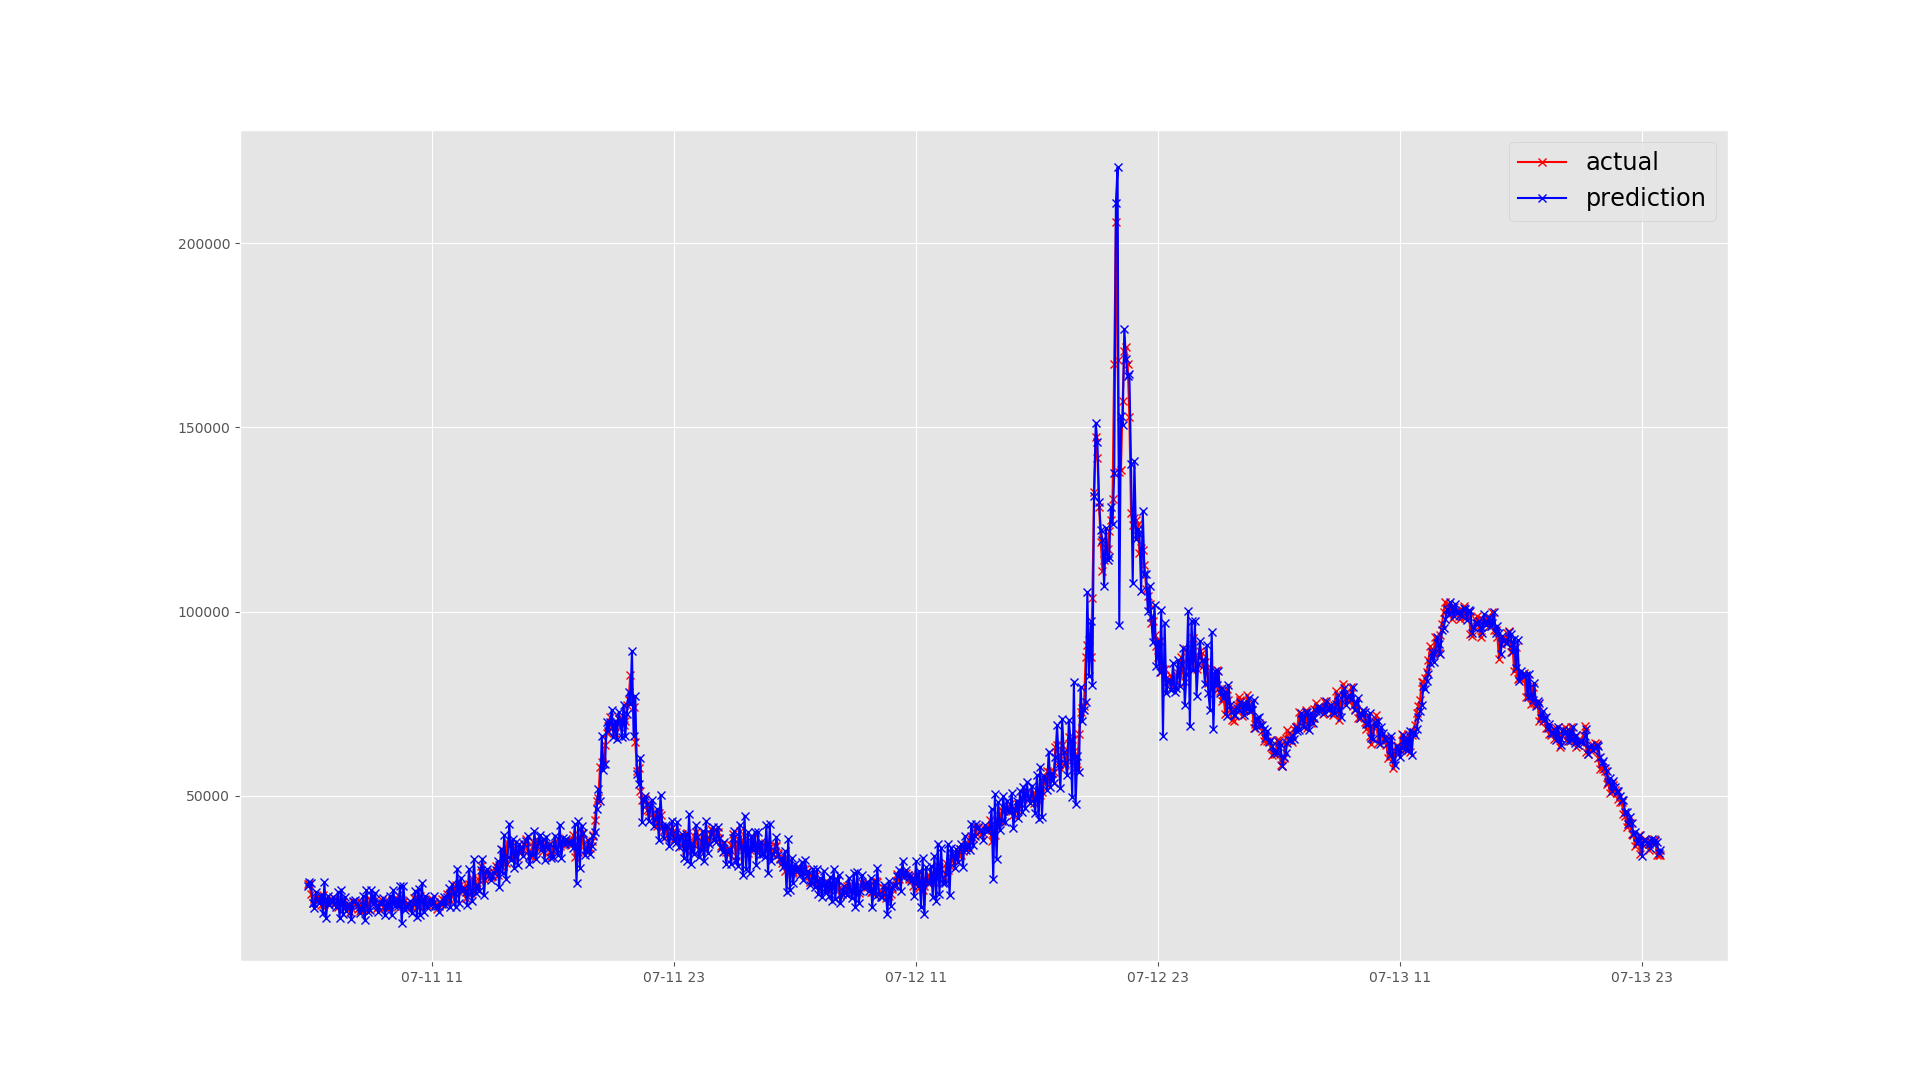
\includegraphics[width=0.45\textwidth]{./figure/arma7379}}
\bicaption[fig:arma_algo]{基于整合移动平均自回归模型的预测}{基于整合移动平均自回归模型的预测结果}{Fig}{The load prediction of ARIMA}
\end{figure}

表\ref{tb:arma}从预测正确率、预测偏差率和预测偏方差率这三个角度显示了基于整合移动平均自回归模型的预测算法对四个不同时间段内流量的实际预测结果:
\begin{table}[h]
\centering
\bicaption[tb:arma]{基于整合移动平均自回归模型的预测算法评估}{基于整合移动平均自回归模型的预测算法评估}{Table}{The precision of prediction for loads based on ARIMA model}
\begin{tabular}{@{}lcccc@{}}\toprule
  & 6.18到6.19 & 6.24 & 7.8到7.9 & 7.11到7.13 \\ \midrule
 预测正确率 & 47.9\% & 45.2\% & 48.0\% & 49.1\% \\
 预测偏差率 & 3.7\% & 5.2\% & 7.0\% & 7.2\% \\
 预测偏方差率 & 7.5\% & 10.3\% & 14.2\% & 14.4\% \\ \bottomrule
\end{tabular}
\end{table}

由表\ref{tb:arma}可知,基于整合移动平均自回归模型的预测算法对上述四个时间段的负载预测精度大体相似,在负载波动稳定的场景下准确率较高,但是在7月8日到7月13日之间出现负载大幅变化的场景下,该预测算法的预测稳定性明显下降。整体而言,基于整合移动平均自回归模型的预测算法在98年世界杯网站访问量的数据集上,整体的预测正确率和预测稳定性都在一个可以接受的范围之内。

\subsection{基于长短期记忆模型的预测实验}\label{sec:lstm_eval}
由于基于长短期记忆模型的预测模型需要先基于一段时间的历史数据先进行离线训练,然后根据训练得出的模型预测下一个周期的资源使用量,我们选择基于5月1日到6月17日之间的历史数据进行训练,并根据此次训练所得的模型进行后续的负载预测计算。图\ref{fig:arma_algo}显示了我们利用基于长短期记忆模型的预测算法,对6月18日到6月19日之间、6月24日当天、7月8日到7月9日之间和7月11日到7月13日期间的流量数据进行预测的结果:
\begin{figure}[htbp]
\centering
\subfigure[6月18日到6月19日]{
    \label{fig:lstm_algo:5255}
    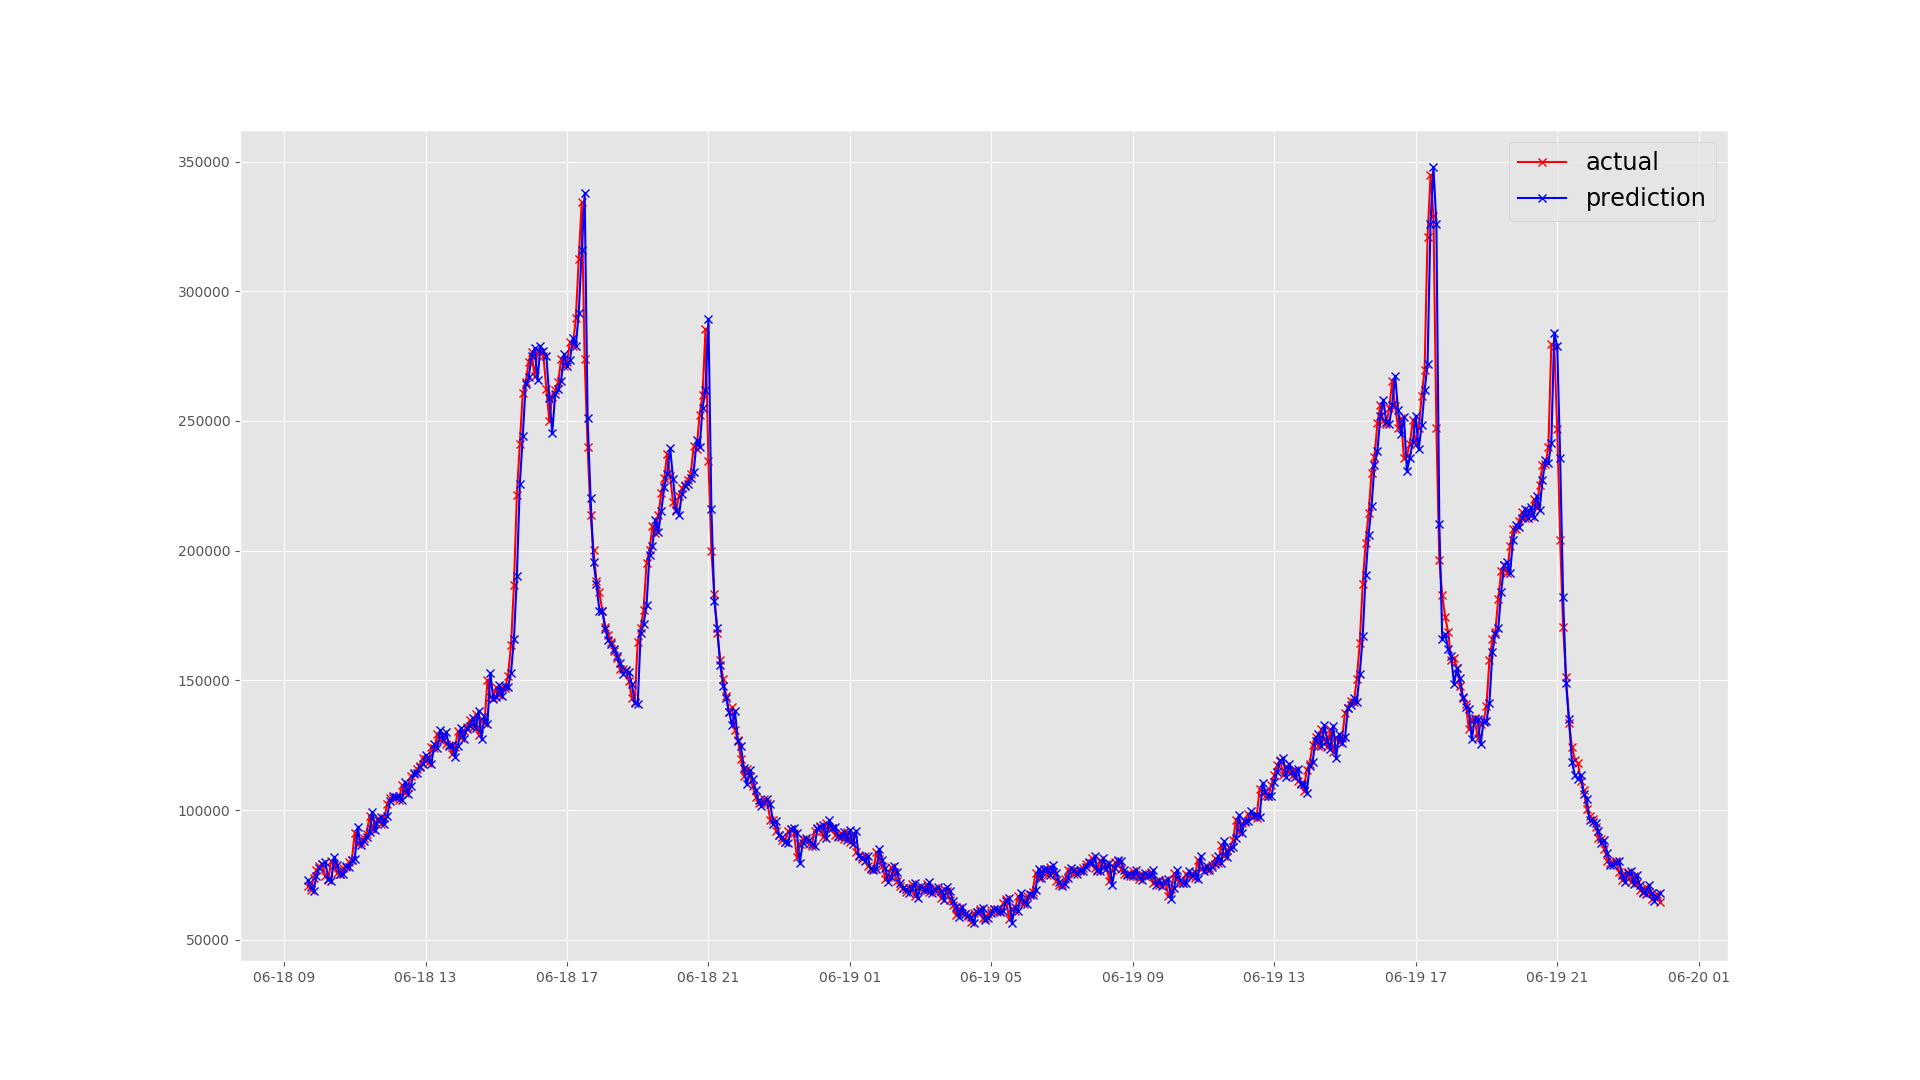
\includegraphics[width=0.45\textwidth]{./figure/lstm5255}}
\subfigure[6月24日]{
    \label{fig:lstm_algo:5961}
    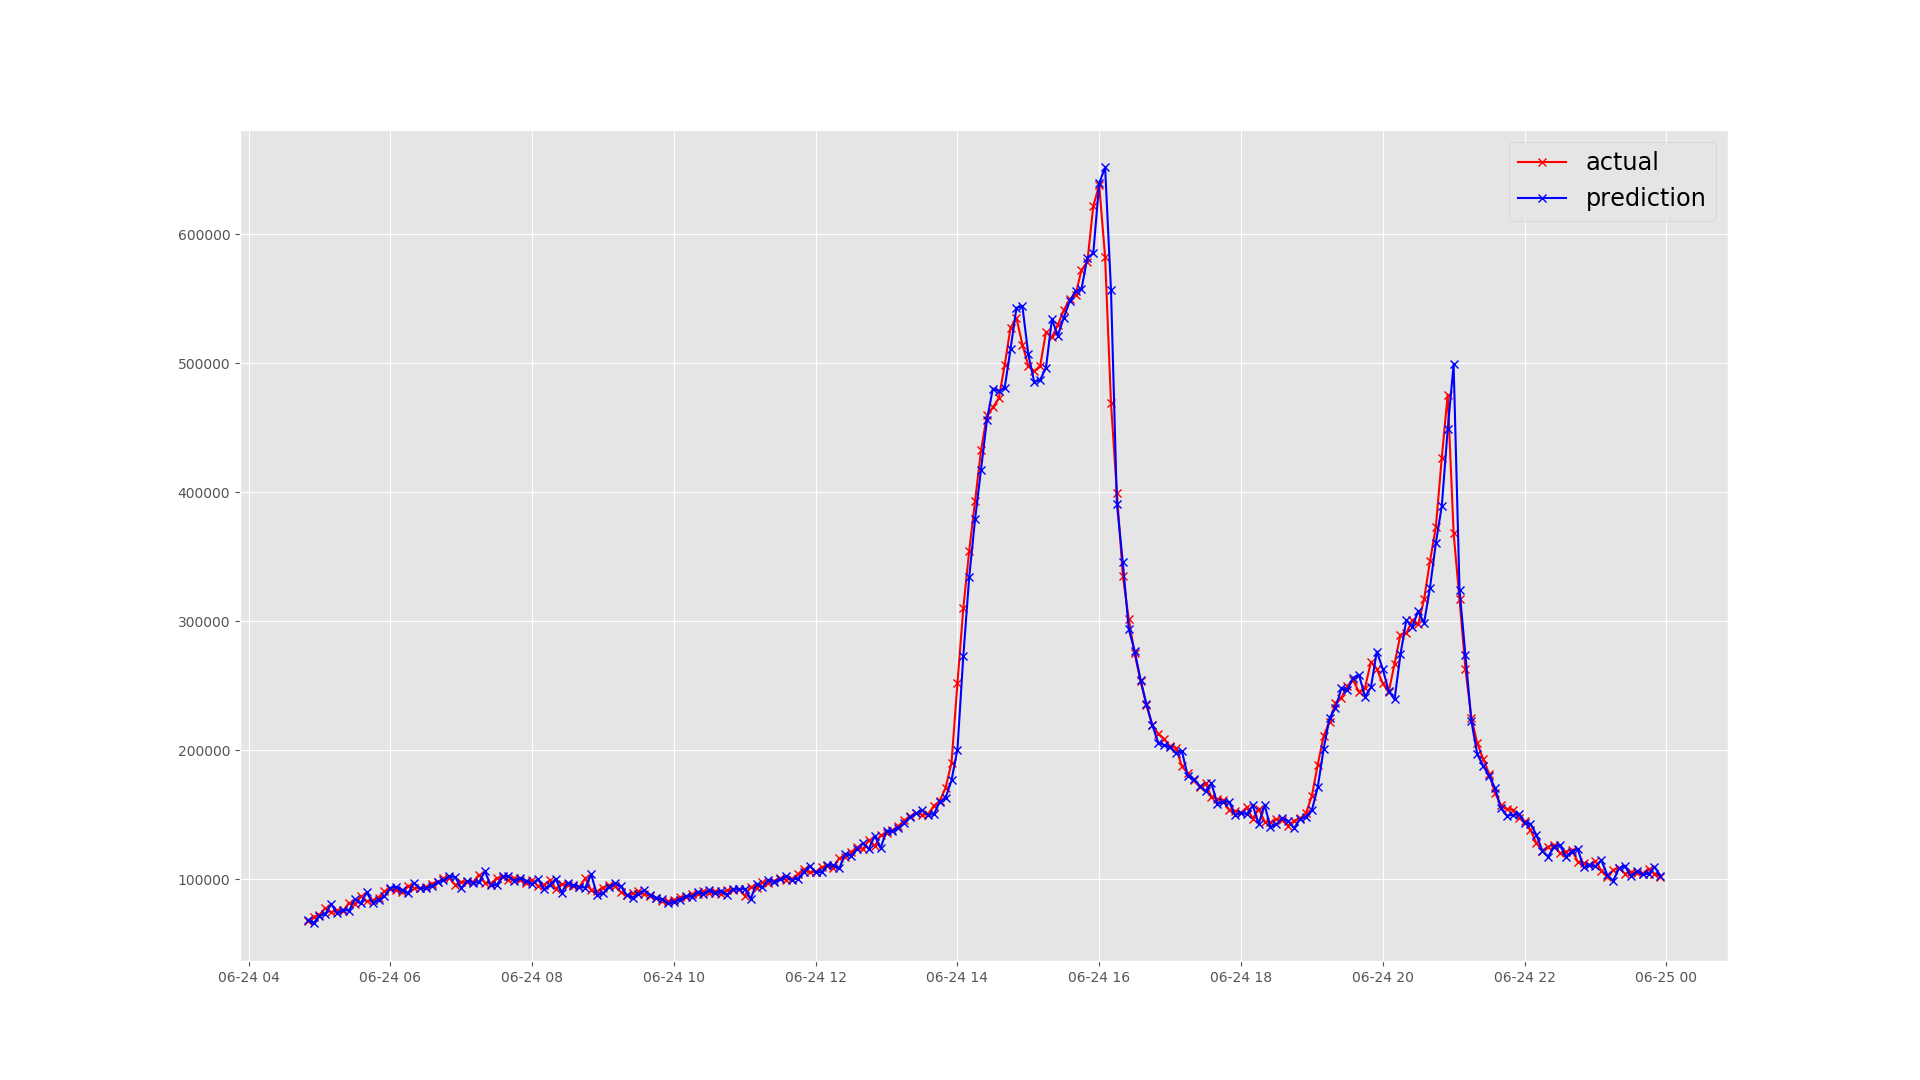
\includegraphics[width=0.45\textwidth]{./figure/lstm5961}}
\subfigure[7月8日到7月9日]{
    \label{fig:lstm_algo:7376}
    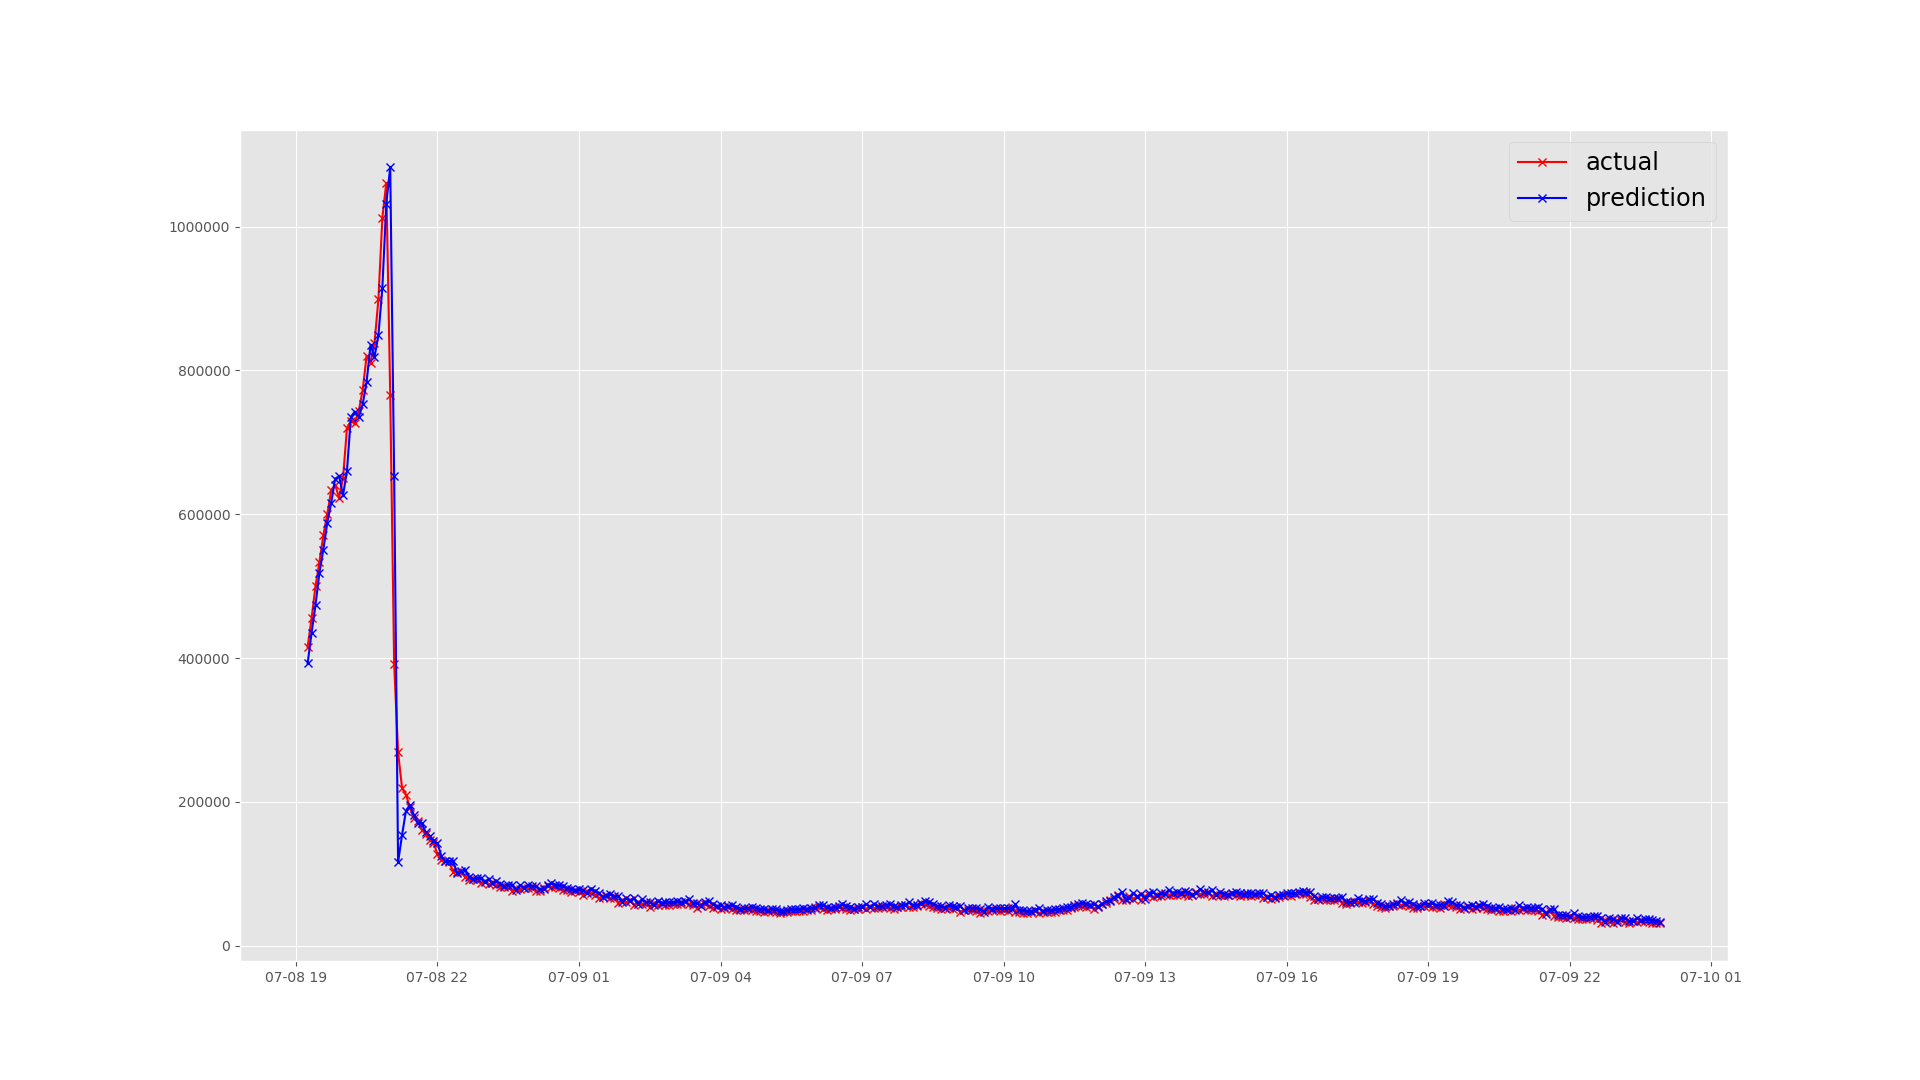
\includegraphics[width=0.45\textwidth]{./figure/lstm7376}}
\subfigure[7月11日到7月13日]{
    \label{fig:lstm_algo:7379}
    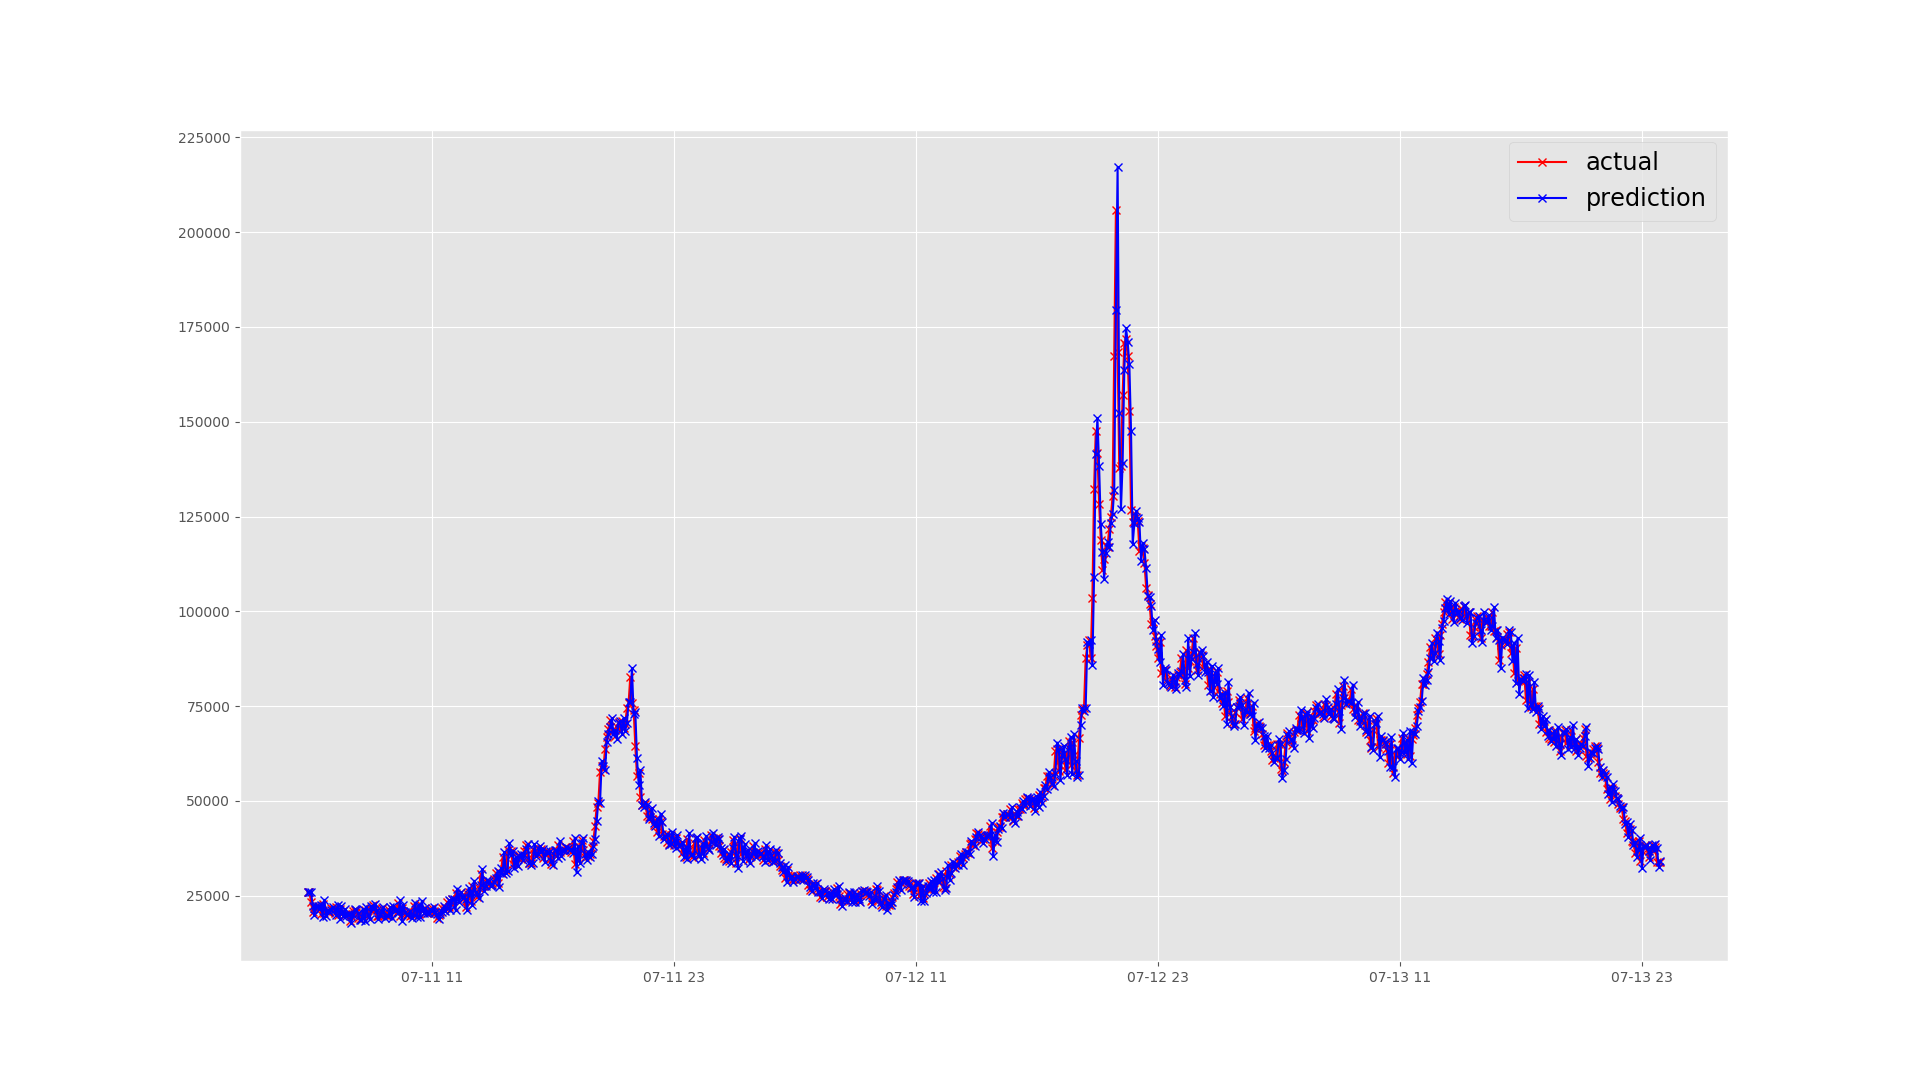
\includegraphics[width=0.45\textwidth]{./figure/lstm7379}}
\bicaption[fig:lstm_day]{基于长短期记忆模型的预测}{基于长短期记忆模型的预测结果}{Fig}{The load prediction of LSTM}
\end{figure}

表\ref{tb:lstm}从预测正确率、预测偏差率和预测偏方差率这三个角度显示了基于长短期记忆模型的预测算法对四个不同时间段内流量的实际预测结果:
\begin{table}[h]
\centering
\bicaption[tb:lstm]{基于长短期记忆模型的预测算法评估}{基于长短期记忆模型的预测算法评估}{Table}{The precision of prediction for loads based on LSTM model}
\begin{tabular}{@{}lcccc@{}}\toprule
  & 6.18到6.19 & 6.24 & 7.8到7.9 & 7.11到7.13 \\ \midrule
 预测正确率 & 44.1\% & 42.2\% & 83.8\% & 49.6\% \\
 预测偏差率 & 3.4\% & 3.5\% & 6.6\% & 4.8\% \\
 预测偏方差率 & 6.8\% & 7.1\% & 13.8\% & 9.5\% \\ \bottomrule
\end{tabular}
\end{table}

我们从表\ref{tb:lstm}中可以发现,基于长短期记忆模型的预测算法对7月8日到7月9日之间的负载数据在预测正确率上出现了明显抖动。这主要是由于7月8日当天的负载骤降的程度超过之前学习的历史数据中所有的骤降记录,因此相对实际的负载状态,预测的结果具有一定的滞后性。除此之外,经过和基于整合移动平均自回归模型的预测实验结果对比,我们发现基于长短期记忆模型的预测算法的预测结果稳定性更好,整体的预测偏差相比基于整合移动平均自回归模型的预测偏差更小,受周期变化的影响更小,从最终的预测效果而言略好于基于整合移动平均自回归模型的预测算法。

\section{负载优化模块有效性验证和分析}
本课题主要目标是使容器云能够更加快速的相应变化的负载,因此除了通过上述的预测来进行提前准备之外,还需要对实时变化的负载进行应对,避免因为预测错误而导致响应延迟,进而降低整体的服务质量。为了验证本课题所提出提出模型的有效性,我们分别从服务的创建和伸缩两个方面进行实验,记录这两个过程中服务调整的时间延迟,通过和Docker \emph{swarm}中的延迟时间进行比较来证明负载优化模块的有效性。我们在本次实验中并没有对服务的销毁进行单独的实验验证,这主要是因为相比于服务的创建而言,服务的销毁更加简单,除了需要从管理者节点同步地清理服务的元信息之外,服务的销毁可以被当作是将服务将实例规模减少到0的操作。

\subsection{服务创建实验}\label{sec:serv_creation}
我们分别使用Docker \emph{swarm}和本课题实现的系统就容器集群中服务创建的过程展开实验。我们针对在容器云中创建服务的测试设计了三个不同的测试场景,并按照\ref{req:serv_aval}中的要求基于应用镜像\emph{image1}、\emph{image2}和\emph{image3}分别创建\emph{service1},\emph{service2}和\emph{service3}这三个服务:
\begin{enumerate}
\item\label{create1} 分别用Docker \emph{swarm}和本课题实现的系统创建服务\emph{service1},\emph{service2}和\emph{service3}。每个服务有2个任务实例,同时为了满足\ref{req:serv_aval}中提到的可用性要求,在本课题实现的系统中为每个服务设置2个副本。
\item\label{create2} 分别用Docker \emph{swarm}和本课题实现的系统依次创建服务\emph{service1},\emph{service2}和\emph{service3}。每个服务有4个任务实例,同时为了满足\ref{req:serv_aval}中提到的可用性要求,在本课题实现的系统中为每个服务设置2个副本。
\item\label{create3} 分别用Docker \emph{swarm}和本课题实现的系统按照\emph{service1},\emph{service3}和\emph{service2}的顺序依次创建相应的服务。每个服务有2个任务实例,同时为了满足\ref{req:serv_aval}中提到的可用性要求,在本课题实现的系统中为每个服务设置2个副本。
\end{enumerate}

我们将测试场景\ref{create1}中的测试结果作为衡量不同服务在本文实现的系统中创建启动相应服务所需耗时的基准值,相应的实验结果如图\ref{fig:baseline}所示:
\begin{figure}[H]
\centering
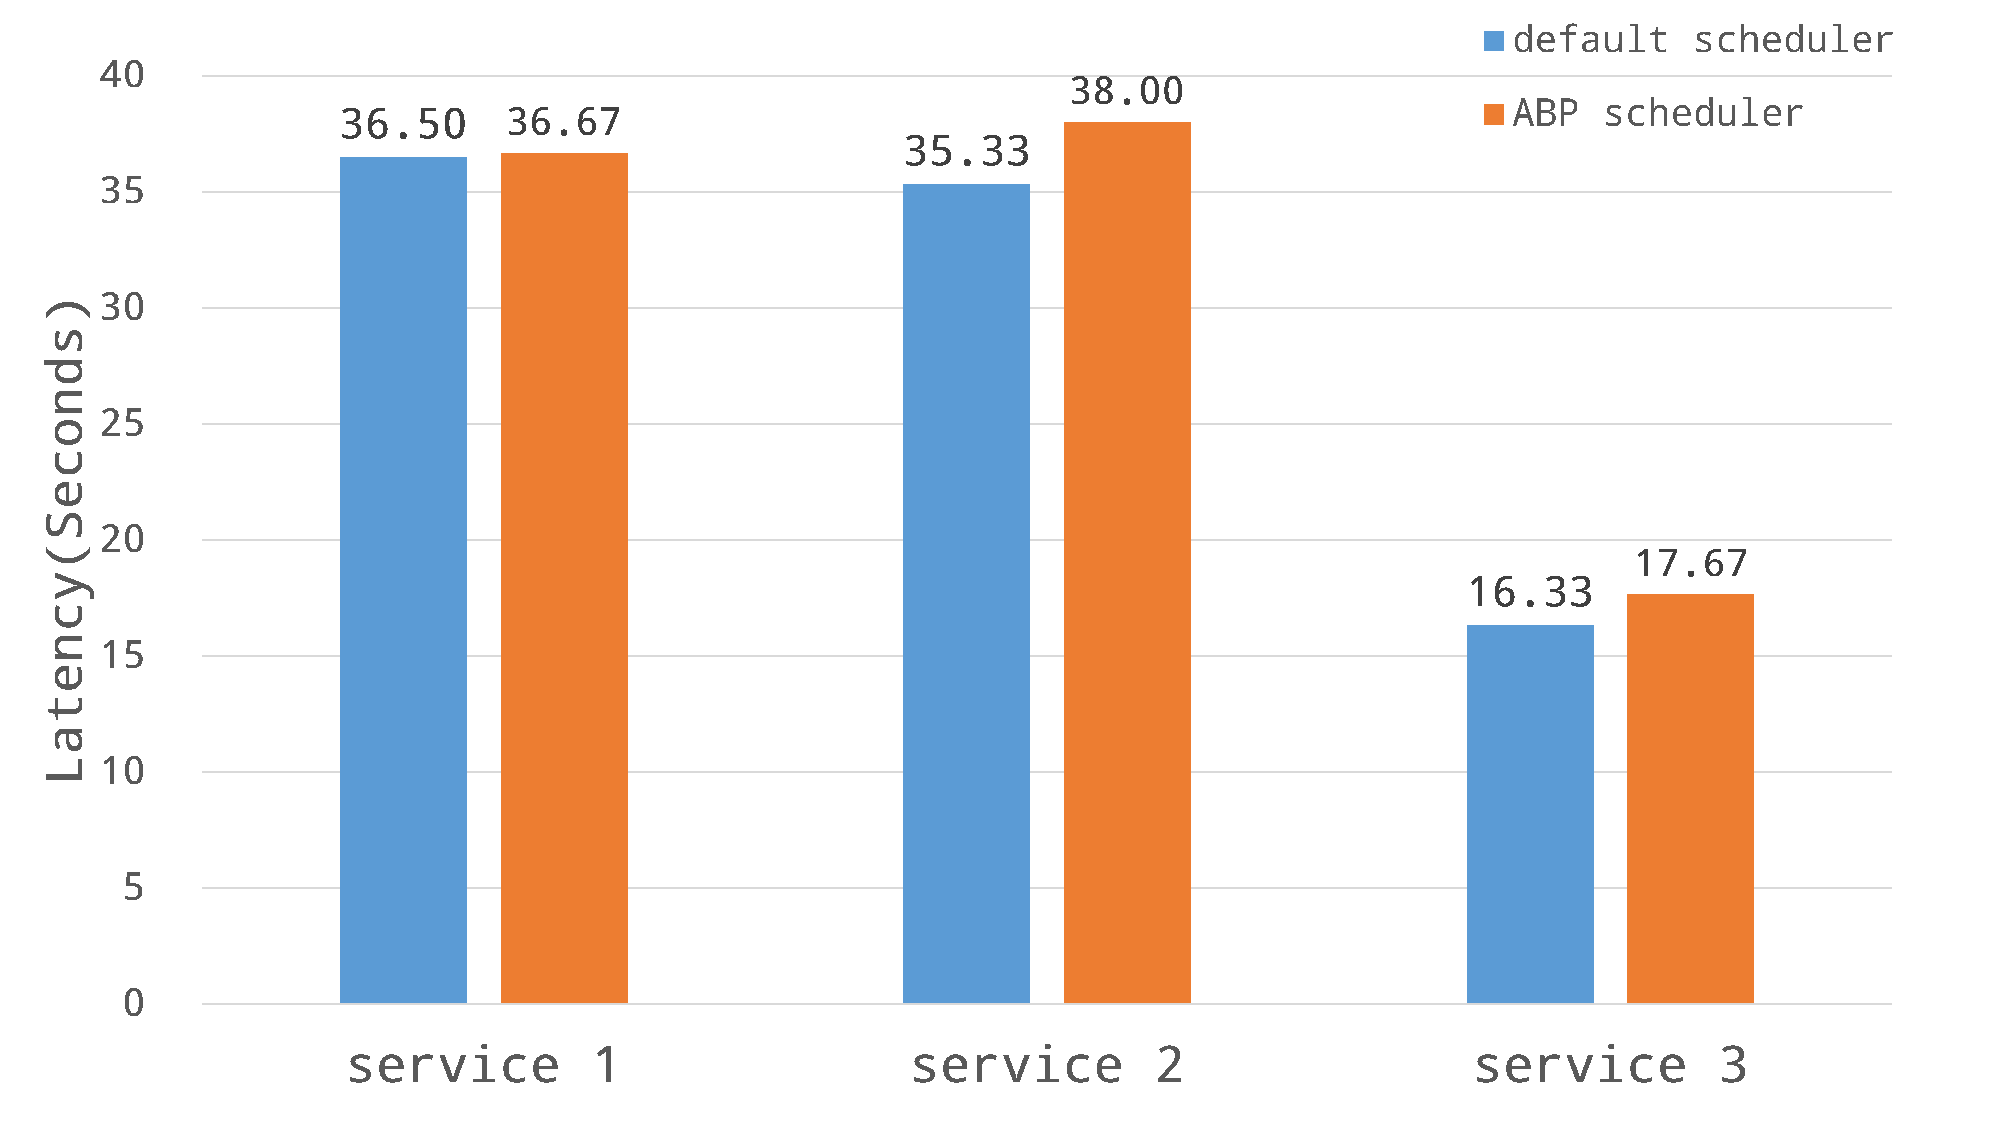
\includegraphics[width=0.9\textwidth]{./figure/baseline}
\bicaption[fig:baseline]{创建服务耗时基准}{\textbf{服务创建耗时}: 以每个服务的副本数要求为2且有2个任务实例作为本次实验的基准}{Fig}{\textbf{Services Creation}: creating each service with 2 tasks and 2 replicas, as the baseline of our experiments}
\end{figure}

从图\ref{fig:baseline}中可以看出,相关服务在我们实现的系统中启动耗时相比默认的Docker \emph{swarm}框架要略微高一些。这是由于相比Docker \emph{swarm}框架,本课题实现的系统需要额外从Docker \emph{registry}服务(并非本地的Docker \emph{registry}镜像服务)通过Docker \emph{Registry} API来获取Docker镜像文件的元数据,因此产生了相应的延迟。但由于镜像元数据中只有各个层级文件的数字签名信息,包含的数据量很小,因此这个额外耗时主要消耗在建立网络连接过程。我们在实验中通过多次测试验证,获取镜像元数据的延迟平均只有1.2秒,整个过程耗时很少超过3秒。对比下载整个镜像文件的耗时造成的延迟损失,我们认为这部分的延迟开销是可以接受的。除此之外,通过对实验观测到的数据进行分析,我们发现本系统中时间延迟的标准差比Docker \emph{swarm}框架中时间延迟的标准差高出1秒左右,这主要是由于从国内实验环境连接到位于美国的Docker \emph{registry}服务的网络环境不稳定导致的。

图\ref{fig:4ins}显示了在测试场景\ref{create2}中我们的系统和Docker \emph{swarm}框架对相应服务执行服务创建操作所需要的时间延迟。
\begin{figure}[H]
\centering
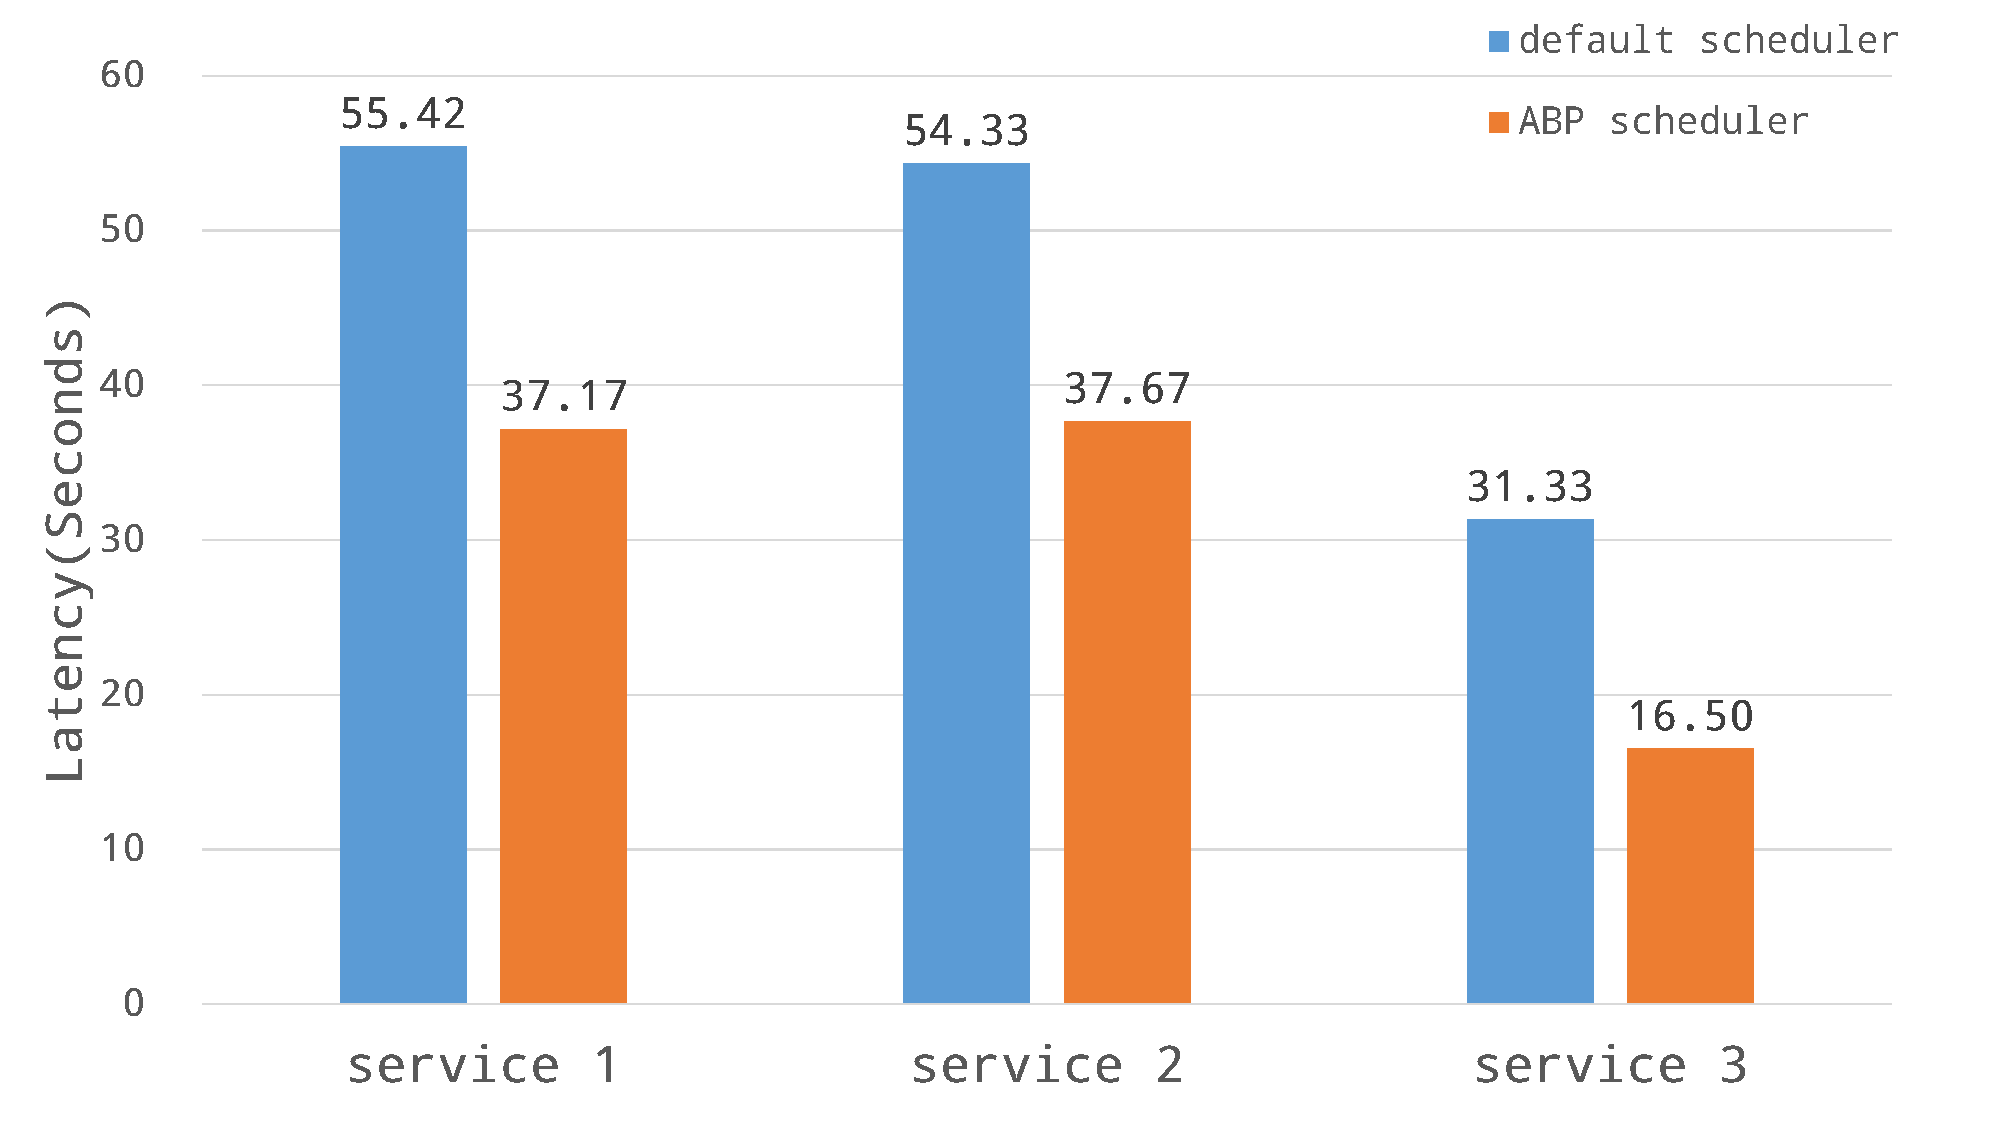
\includegraphics[width=0.9\textwidth]{./figure/4ins2rep}
\bicaption[fig:4ins]{创建服务:每个服务副本数要求为2且有4个任务实例}{\textbf{服务创建耗时}:每个服务副本数要求为2且有4个任务实例}{Fig}{\textbf{Services Creation}: creating each service with 4 tasks and 2 replicas}
\end{figure}

从图\ref{fig:4ins}中可知,在测试场景\ref{create2}下,服务在容器云中通过本课题实现的系统比通过Docker \emph{swarm}框架能以更快的速度完成创建和启动。对比图\ref{fig:4ins}和图\ref{fig:baseline},我们可以发现随着任务实例数的增加,Docker \emph{swarm}框架需要接近两倍于基准的延迟等待时间来完成相应服务的创建启动过程。Docker \emph{swarm}框架中服务启动出现大幅度延迟的原因是容器集群和本地Docker \emph{registry}镜像服务间的网络带宽。根据在之前的实验环境\ref{req:registry_mirror},容器集群和本地Docker \emph{registry}镜像服务间的网络带宽为100Mbps。在测试场景\ref{create2}下,每个服务在容器云中有4个任务实例需要创建并运行。在Docker \emph{swarm}框架下,每个服务的4个任务实例被平均分配到集群的4个节点上,集群内的网络请求数目随着实例数目增长而增长(最多可达到集群内的节点数目)。当这4个节点接受了对应的任务实例后,节点上的Docker Engine会开始从本地Docker \emph{registry}镜像服务获取相应的Docker镜像。在测试场景\ref{create1}下,由于每个服务只有2个任务实例,所以每次服务创建时只有两个镜像下载请求来平分容器集群和本地Docker \emph{registry}镜像服务间的网络带宽。在测试场景\ref{create2}中,因为有4个镜像下载请求同时存在,导致网络带宽由原来被2个下载请求平分变成被4个下载请求平分。网络请求数目增加了一倍,使得每个下载请求的传输速度只有测试场景\ref{create1}中的一半,导致整体下载耗时增加了一倍。与Docker \emph{swarm}框架相反,在本课题实现的系统中,为了满足服务自身的可用性目标,每个服务的4个任务实例被分配到了集群内的2个节点上。这使得系统在满足服务可用性要求的前提下,整个容器集群中只有两个节点发出下载请求使用网络。容器集群和本地Docker \emph{registry}镜像服务间的100Mbps网络带宽在实验场景\ref{create1}中和实验场景\ref{create2}中都是同时被两个下载请求平分,并没有增加集群内的网络流量。每个下载请求的传输速度没有变化,因此服务整体的启动延迟在实验场景\ref{create2}中和实验场景\ref{create1}中几乎一致。

在实际进行服务创建时,通过对初始状态的负载进行分析,相比于满足可用性目标的副本数目,服务往往需要更多的实例来应对初始负载需要来保证服务本身的质量。为了评估本课题实现的系统在该场景下的表现,我们设计了实验场景\ref{create3}并进行了相关实验,实验结果如图\ref{fig:132}所示:
\begin{figure}[H]
\centering
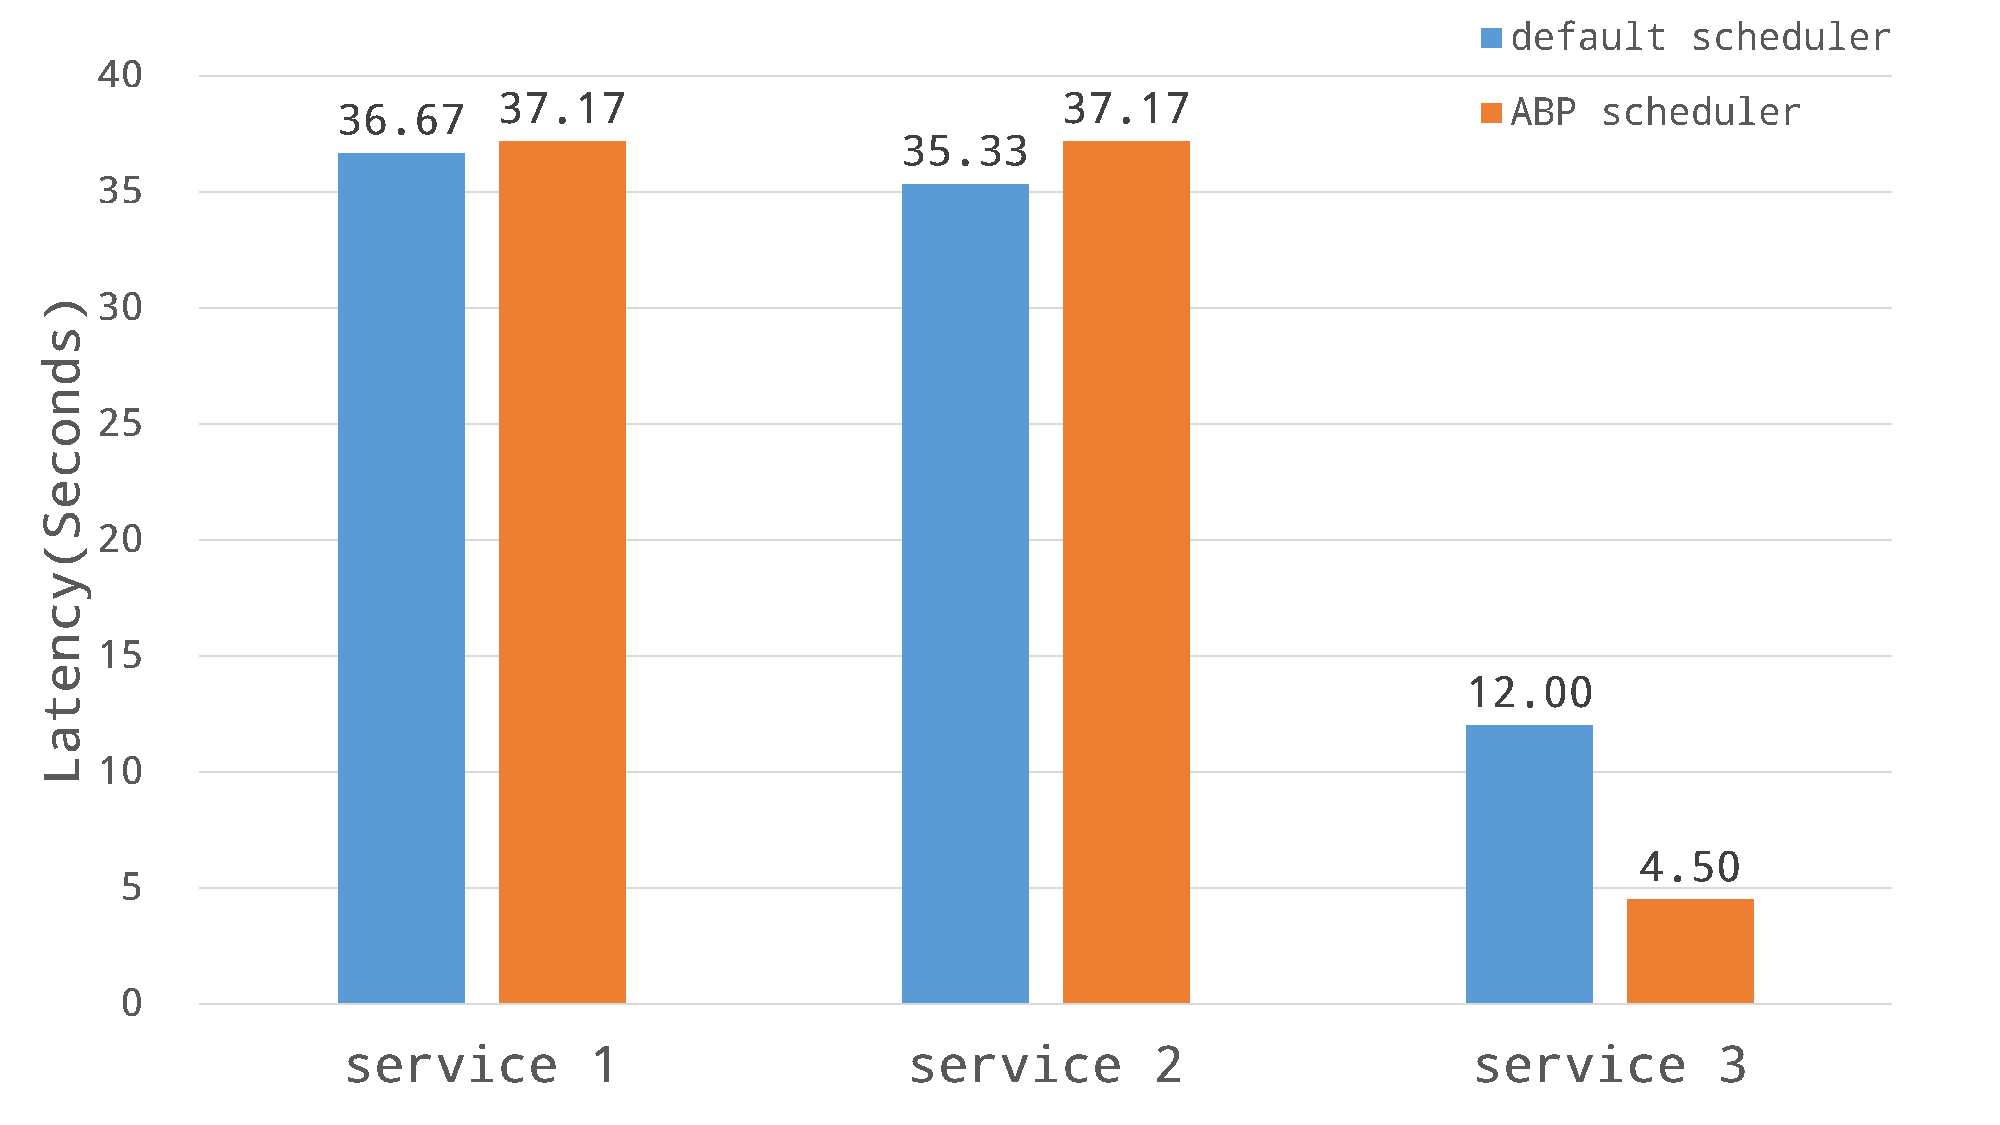
\includegraphics[width=0.9\textwidth]{./figure/132}
\bicaption[fig:132]{按照\emph{service1},\emph{service3}和\emph{service2}的顺序依次创建服务:每个服务副本数要求为2且有2个任务实例}{\textbf{服务创建耗时}: 每个服务副本数要求为2且有2个任务实例,按照\emph{service1},\emph{service3}和\emph{service2}的顺序依次创建各个服务}{Fig}{\textbf{Services Creation}: creating services with 2 tasks and 2 replicas in a sequence of \emph{service1}, \emph{service3} and \emph{service2}}
\end{figure}

从图\ref{fig:132}中可以明显看出,服务\emph{service3}整体的启动延迟时间在本课题实现的系统中比在Docker \emph{swarm}框架中存在显著降低。这主要是如我们在第\ref{chap:sys_design}章中所说,因为本课题实现的系统在资源分配阶段考虑了Docker镜像中的层级文件和容器集群节点上保存的Docker镜像文件缓存相关性,在同一节点上的不同服务间共享了部分Docker镜像分层文件缓存,降低了服务在创建和启动方面的延迟。根据我们在前面准备部分\ref{req:serv_image}中相关Docker镜像的具体构成,服务\emph{service1}和服务\emph{service3}使用的应用镜像\emph{image1}和\emph{image3}都包含了来自\emph{debian:jessie}这个基础镜像的同样的层级文件。在服务\emph{service1}被创建的过程中,\emph{debian:jessie}镜像的层级文件会被这些准备运行服务\emph{service1}相关任务实例的集群节点下载并缓存。在对服务\emph{service3}的任务实例基于负载应对选择托管的容器集群节点时,根据在\ref{sec:scheduler}节中的设计,本课题实现的系统将优先把相应任务实例分布到那些已经运行了服务\emph{service1}任务实例的集群节点。此外,我们在实验过程中也发现如果按照\emph{service1}、\emph{service2}和\emph{service3}的顺序创建相关服务,服务\emph{service3}的任务实例在Docker \emph{swarm}框架下有时也会被分发到运行着服务\emph{service1}任务实例的集群节点上。这主要是当集群中节点运行的任务实例数目相同时,Docker \emph{swarm}框架根据节点的通用唯一识别码(Universally Unique Identifier,UUID)按照字典序进行任务的分发和调度,集群中节点的UUID则由节点上的Docker Engine在启动的时候基于\emph{sha256}算法随机生成。

\subsection{服务伸缩实验}\label{sec:serv_scale}
我们已经在第\ref{sec:serv_creation}节中显示了本课题实现的系统在服务创建和启动方面相比Docker \emph{swarm}框架带来的显著提升。虽然服务创建的表现对保障服务质量很重要,但是在动态变化的负载压力下,服务进行伸缩的性能表现则是关键。当负载增长时,服务需要进行扩展(scale-out)以保证服务质量;当负载降低时,服务需要进行收缩(scale-in)从而减少不必要的资源,提高资源使用率,降低成本。降低服务伸缩过程任务实例的启动/关闭延迟可以增强服务整体应对负载变化的灵活性,从而更好地保证服务的质量。为了验证本课题实现的系统在服务扩展和服务收缩场景下对任务实例启动延迟的影响,我们设计了如下两个实验并和Docker \emph{swarm}框架进行了对比:
\begin{enumerate}
\item\label{scale1} 基于服务创建实验\ref{create1}中的要求创建服务,然后将相应的服务扩展到4个任务实例,最后再将相应服务收缩到2个任务实例。对服务\emph{service1},\emph{service2}和\emph{service3}独立进行上述实验,每次实验之前重置整个实验环境,保证不同服务的实验之间没有影响。
\item\label{scale2} 基于服务创建实验\ref{create3}创建服务,分别用Docker \emph{swarm}和本课题实现的系统按照\emph{service1},\emph{service3}和\emph{service2}的顺序依次创建服务。每个服务有2个任务实例,同时为了满足\ref{req:serv_aval}中提到的可用性要求,在本课题实现的系统中为每个服务设置2个副本。随后,将服务\emph{service1}扩展到4个任务实例。
\end{enumerate}

以上两个实验设计均包含了服务的扩展和伸缩部分,但是这两个设计针对的场景侧重点不同。实验设计场景\ref{scale1}主要通过对各个服务的伸缩性能进行独立实验来验证本系统在单一服务场景下对单个服务伸缩性能的影响;验设计场景\ref{scale2}通过从所有服务中选择一个服务来进行伸缩实验从而来验证本系统在多服务的场景下对其中一个服务进行伸缩时的性能影响。以下将根据以上两个设计场景下的实验结果整合后,分为服务扩展和服务收缩两部分进行介绍和说明。

\subsubsection{服务扩展表现}
图\ref{fig:scaleout}显示了相应服务在Docker \emph{swarm}框架中和本文实现的系统中执行服务扩展操作所需要的时间开销。
\begin{figure}[H]
\centering
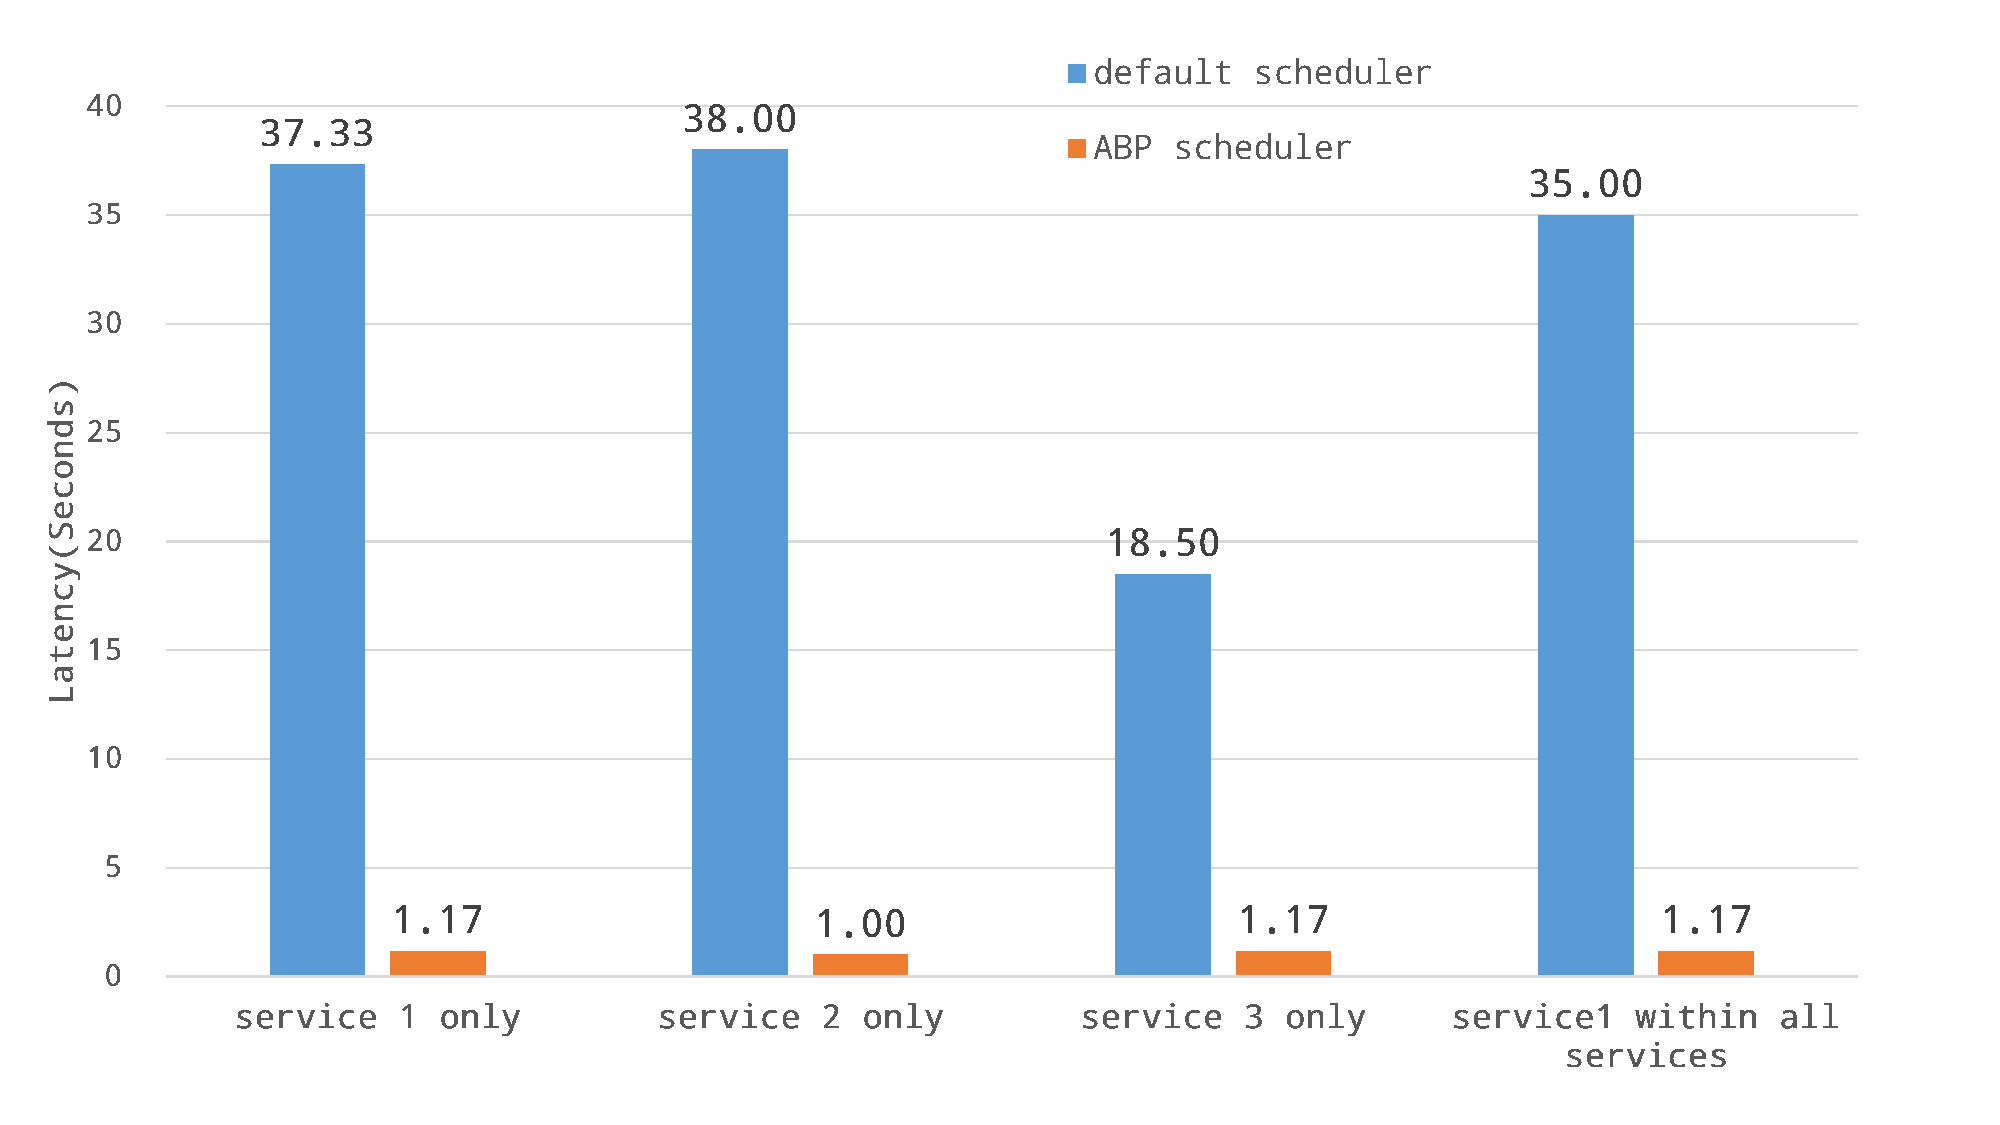
\includegraphics[width=0.9\textwidth]{./figure/scaleout}
\bicaption[fig:scaleout]{服务扩展实验}{\textbf{服务扩展-应对负载增加}}{Fig}{Service Scaling Out}
\end{figure}

图\ref{fig:scaleout}中的实验结果显示出我们实现的系统对服务扩展操作的加速效果十分明显,服务扩展的延迟比在Docker \emph{swarm}框架中有大幅度降低。通过本课题实现的系统,容器云中的服务能在极短的时间延迟(基本不超过2s)下完成伸缩,这显然在负载急剧增长的场景下能对提升服务整体的服务质量有极大的帮助。与之相对,我们发现在Docker \emph{swarm}框架下,每个服务的扩展延迟几乎等于他们创建阶段的耗时,而创建耗时又和服务所使用的Docker镜像大小密切相关。鉴于Docker \emph{swarm}框架中服务的任务实例常常被尽可能平均地分发到了整个容器集群中所有满足限制条件的节点上,使得整个容器集群中的节点上任务实例近似一致。而在整个容器集群中,并不是所有节点都拥有相应服务所依赖的层级文件缓存。这就导致有些任务实例被分发到了一个完全没有任何相关依赖层级文件缓存的集群节点上,而这些节点则需要下载对应服务所需要的完整Docker镜像从而来运行这些任务实例。当服务在本课题实现的系统中需要进行扩展的时候,系统会根据节点上的层级文件缓存和当前服务所需Docker镜像中层级文件的重合度以及节点的资源利用率来从容器集群中选择合适的节点来运行扩展的任务实例。因此在系统中被选择用作运行新任务实例的节点不需要下载全部的Docker镜像文件,加快了扩展任务实例的启动时间,从而降低了服务扩展操作的整体延时。

我们从图\ref{fig:scaleout}中还可以发现:在伸缩实验场景\ref{scale2}下,按照\emph{service1},\emph{service3}和\emph{service2}的顺序创建相应服务后,在Docker \emph{swarm}框架下对服务\emph{service1}进行扩展时,服务扩展操作所需要的耗时相比单独对服务\emph{service1}进行扩展时所要的耗时略有降低。出现降低的原因是在该场景下容器集群中所有节点都在之前的创建过程中缓存了底层基础镜像\emph{debian:jessie}镜像,从而减少了这部分文件下载所需要的耗时。在该场景下,由于集群只有4个节点并且按照\emph{service1}、\emph{service3}和\emph{service2}的顺序依次创建相应的服务,服务\emph{service1}扩展产生的任务实例被分发到集群中尚未运行服务\emph{service1}任务实例的两个节点。根据我们在之前实验环境准备环节\ref{req:serv_image}部分中的设定说明,服务\emph{service1}和服务\emph{service3}使用的应用镜像\emph{image1}和\emph{image3}都使用\emph{debian:jessie}镜像作为基础镜像,因此这两个应用镜像可以共享这部分层级文件的缓存。当我们在伸缩实验场景\ref{scale2}下下对服务\emph{service1}进行扩展的时候,这两个节点上已经运行了服务\emph{service3}的相关任务实例,因此针对\emph{debian:jessie}镜像这一部分的层级文件可以直接利用存储在各自节点上的缓存,而不需要如同对服务单独扩展实验中一样去下载这些层级文件。不过我们从图\ref{fig:scaleout}中也可以发现,即使利用了这部分缓存的共享层级文件,对减少服务扩展操作的延迟而言效果仍然不够显著。在Docker \emph{swarm}框架中,运行扩展任务实例的节点仍然需要下载约270MB大小的层级文件以安装应用运行所需要的\emph{Golang}运行时环境,随后还需要对下载下来的层级文件进行解压缩操作后通过相应的安装指令进行安装。与之相对的是在本课题实现的系统中,运行扩展任务实例的节点由于在本地已经缓存了服务\emph{service1}使用的Docker容器镜像,因此避免了对相应层级文件的下载和安装耗时,同时减少了容器集群内网络开销。

\subsubsection{服务收缩表现}
当服务在Docker \emph{swarm}框架中进行收缩时,Docker \emph{swarm}框架会从所有节点中根据运行该服务相应任务实例数目进行选择并试图将集群中节点上运行的实例数目接近一致。根据本课题在第\ref{sec:scalein}节
中提出的设计思路,本课题实现的系统则根据任务实例的优势资源相对节点总资源的占比进行选择。图\ref{fig:scalein}显示了服务收缩在Docker \emph{swarm}框架和本课题实现的系统中所需要的延迟:
\begin{figure}[H]
\centering
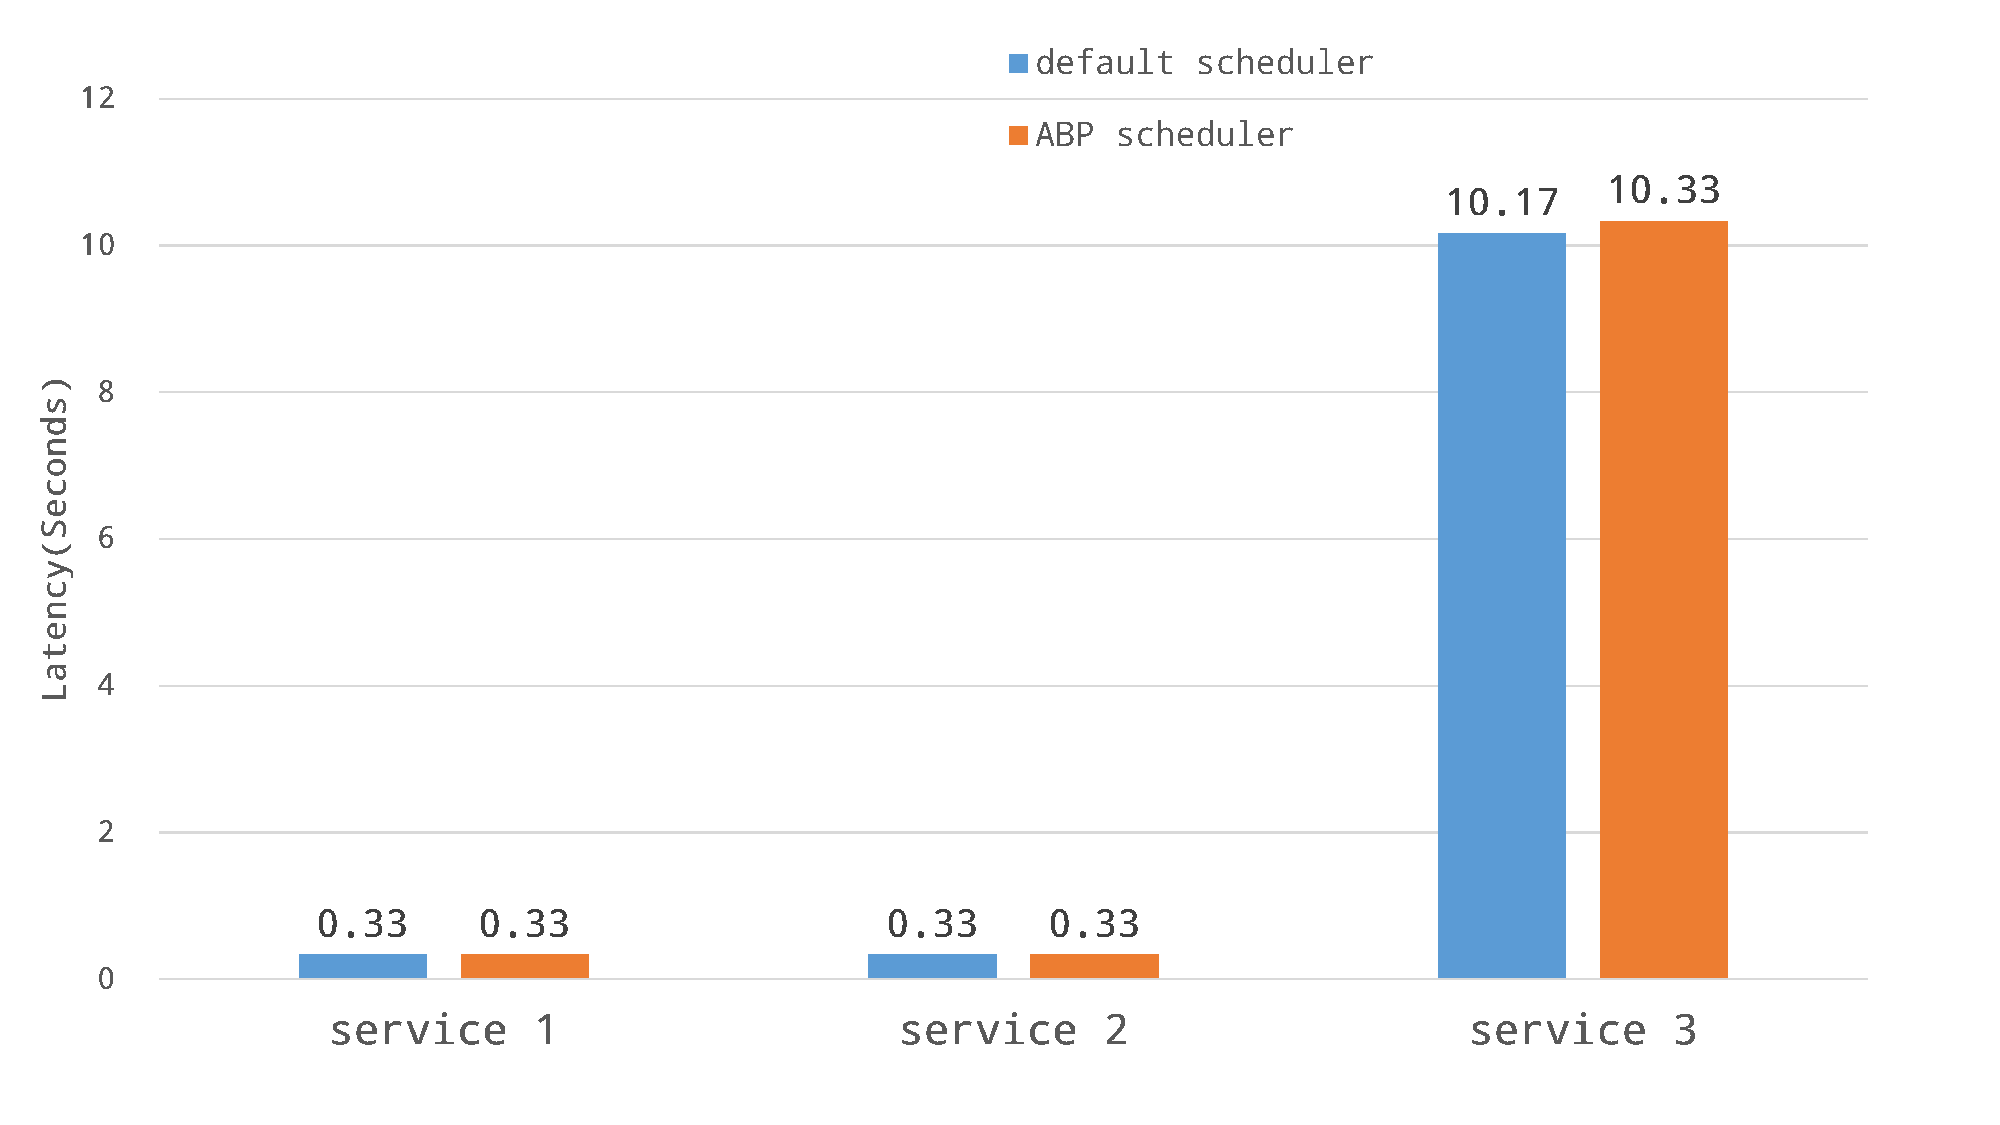
\includegraphics[width=0.9\textwidth]{./figure/scalein}
\bicaption[fig:scalein]{服务收缩实验}{\textbf{服务收缩-应对负载降低}}{Fig}{Service Scaling In}
\end{figure}

我们由图\ref{fig:scalein}可以发现,在Docker \emph{swarm}框架和我们实现的系统中几乎都是立即完成了相应的服务收缩操作,收缩操作的时间延迟基本不超过0.5秒。服务\emph{service3}的收缩操作延迟相比其他两个服务显得很异常,但是也这是在预期之中的。这主要是因为服务\emph{service3}运行的是一段包含了无限循环的shell脚本,导致运行相应任务实例的容器无法响应该节点上的Docker Engine正常发送的停止请求。根据Docker Engine中定义的容器关闭规则,在经过一个既定的等待期(默认10秒)之后,Docker Engine将通过发送SIGKILL的方式强制杀死运行对应任务实例的容器进程。通过对比,我们可以发现服务在Docker \emph{swarm}框架和本课题实现的系统中进行收缩需要的延迟几乎毫无差别。

\section{本章小结}
在本章中,我们从负载预测的准确性和新任务实例调度策略对容器云中任务实例分发管理的影响这两个方面进行实验,并通过这两方面实验的结果对本文提出的基于容器的主动式云资源管理模型的有效性进行验证和讨论。我们使用1998年世界杯网站的负载记录来模拟实际的云中资源负载状态,并通过实验的结果证明资源使用状态预测模块可以提供有效可靠的预测结果。通过服务创建和服务伸缩的实验结果证明,在负载急剧增加的场景下,本文提出的模型显著加快了服务在容器云中的扩展速度;而在负载降低的场景下,本文提出的模型保证了服务收缩的操作和Docker \emph{swarm}中的服务收缩一样高效。我问提出的模型通过有效地结合基于负载预测的调整和优化服务伸缩调整的延迟,最终实现提高对负载变化的响应能力。
